% -*- Mode:TeX -*-

%% The documentclass options along with the pagestyle can be used to generate
%% a technical report, a draft copy, or a regular thesis.  You may need to
%% re-specify the pagestyle after you \include  cover.tex.  For more
%% information, see the first few lines of sk-thesis.cls. 

% DRAFT MODE uses simpler front page, without dedication, acknowledgements, uses a footer sying draft.
%\documentclass[12pt,a4paper,vi,twoside,leftblank]{sk-thesis}
%\documentclass[12pt,a4paper,vi,draft]{sk-thesis}
\documentclass[12pt,a4paper,vi]{sk-thesis}
\usepackage[utf8]{inputenc}
\usepackage{geometry}
\usepackage{amsmath}
\geometry{a4paper, right=15mm, bottom=20mm, left=30mm, top=20mm}

\usepackage{ifdraft}
\usepackage{graphicx}
\setkeys{Gin}{draft=false} % disable hiding graphics in draft mode
\usepackage[table]{xcolor}
\usepackage{multicol, multirow}
\usepackage{amsmath, amssymb}
\usepackage{cmap}
\usepackage[T1]{fontenc}
\setlength {\marginparwidth }{2.5cm} 
\usepackage[obeyDraft]{todonotes}
\usepackage{booktabs, siunitx}
\usepackage[breaklinks=true]{hyperref}
\usepackage{breakcites}
\usepackage[nottoc,numbib,numindex]{tocbibind}
\usepackage[numbers]{natbib} 
\usepackage{bibentry}
\usepackage{doi}
\definecolor{navyblue}{rgb}{0.0, 0.0, 0.5}
%\definecolor{royalblue}{rgb}{0.06, 0.11, 0.42}
\hypersetup{
  final,
  colorlinks=true,
  urlcolor=navyblue,
  citecolor=navyblue,
  linkcolor=navyblue
}
\usepackage{cleveref}
\crefformat{footnote}{#2\footnotemark[#1]#3}
\usepackage{catoptions}
\makeatletter
%\def\figureautorefname{figure}
%\def\tableautorefname{table}
\def\Autoref#1{%
  \begingroup
  \edef\reserved@a{\cpttrimspaces{#1}}%
  \ifcsndefTF{r@#1}{%
    \xaftercsname{\expandafter\testreftype\@fourthoffive}
      {r@\reserved@a}.\\{#1}%
  }{%
    \ref{#1}%
  }%
  \endgroup
}
\def\testreftype#1.#2\\#3{%
  \ifcsndefTF{#1autorefname}{%
    \def\reserved@a##1##2\@nil{%
      \uppercase{\def\ref@name{##1}}%
      \csn@edef{#1autorefname}{\ref@name##2}%
      \autoref{#3}%
    }%
    \reserved@a#1\@nil
  }{%
    \autoref{#3}%
  }%
}
\makeatother
\usepackage{textcomp}
\usepackage{fancyhdr}
\newcommand{\changefont}{%
    \fontsize{10}{10}\selectfont
}
\fancyhf{}
%\fancyhead[LE]{\slshape \rightmark} %section
%\fancyhead[RE]{}
%\fancyhead[RO]{\slshape \leftmark} % chapter
%\fancyhead[LO]{}
\fancyhead[LE,RO]{\changefont \slshape \nouppercase{\rightmark}} %section
\fancyhead[RE,LO]{\changefont \slshape \nouppercase{\leftmark}} %chapter
\fancyfoot[C]{\thepage} %footer
\usepackage{datetime}
\usepackage[automake,toc]{glossaries}
\glsenablehyper
\makeglossaries
%\usepackage{comment}
\usepackage{subcaption}
\usepackage{tabularx, lscape, rotating}
\usepackage[most]{tcolorbox}
\newtcolorbox{myframe}[1][]{
  enhanced,
  top=12pt,bottom=12pt,left=16pt,right=16pt,
  arc=0pt,
  outer arc=0pt,
  colback=white,
  boxrule=1pt,
  #1
}

%%%%%%%%%%%% EPIGRAPH
\usepackage{epigraph}
%\setlength{\beforeepigraphskip}{1.0\baselineskip}
\setlength{\epigraphrule}{0pt}
\setlength{\epigraphwidth}{.4\textwidth}
%\setlength{\afterepigraphskip}{.25\baselineskip}
\renewcommand{\textflush}{flushepinormal}

% multiline table columns
\usepackage{array}
\newcolumntype{L}{>{\centering\arraybackslash}m{8cm}}
% https://stackoverflow.com/questions/790932/how-to-wrap-text-in-latex-tables
    
\ifdraft{
    %% LIMIT CHAPTERS
    \includeonly{
        prelude,
        contents,
        chapters/introduction,
        chapters/background,
        chapters/roadmap,
        chapters/thesis-objectives,
        chapters/methodology,
        chapters/conclusion,
        glossary,
        bibliography,
        chapters/appendix-a
    }
}{
}

\begin{document}

\ifdraft{
    %%%%%%%%%%% HEADERS AND FOOTERS
    \fancypagestyle{plain}{%
      \fancyhf{}%
      \renewcommand{\headrulewidth}{0pt}% Line at the header invisible
      \fancyfoot[L]{\changefont PhD Thesis - Student Name} % DRAFT ONLY
      \fancyfoot[C]{\thepage}% \changefont 
      \fancyfoot[R]{\changefont \textbf{DRAFT} \today} % DRAFT ONLY
    }
    \fancyfoot[L]{\changefont PhD Thesis - Student Name} % DRAFT ONLY
    \fancyfoot[R]{\changefont \textbf{DRAFT} \today} % DRAFT ONLY
    \pagestyle{fancy}
    
    %% SIMPLE TITLE PAGE
    \chapter*{Thesis Title}

\begin{center}
\Large{
\textsc{PhD Thesis (Final Draft) \\ Student Name \\ }
}

\today\ 
% \currenttime
\end{center}

\clearpage

\section*{Abstract}
\kant[1-2]

%\section*{Publications}
\subsection*{Main author}
\nobibliography*
\begin{enumerate}
    \item \bibentry{Skoltech2017}
\end{enumerate}

\subsection*{Co-author}
\begin{enumerate}
    \item \bibentry{Skoltech2017}
\end{enumerate}

\listoftodos
\clearpage
}{
    %% FULL TITLE PAGE
    % -*-latex-*-
% NOTE:
% These templates make an effort to conform to the Skoltech Thesis specifications,
% however the specifications can change.  We recommend that you verify the
% layout of your title page with your thesis advisor and the Education department 
% before printing your final copy.
\title{Indoor SLAM based on crowdsourced data with multiple smartphone sensors}

\author{Timur Chikichev}
% If you wish to list your previous degrees on the cover page, use the 
% previous degrees command:
%       \prevdegrees{MSc, University of Salzburg (2007)}
% You can use the \\ command to list multiple previous degrees
%       \prevdegrees{B.S., University of California (1978) \\
%                    S.M., Massachusetts Institute of Technology (1981)}
\department{Skoltech Center of Research, Entrepreneurship and Innovation}

\degree{Master Program in Space and Engineering Systems}

\degreemonth{November}
\degreeyear{2021}
\thesisdate{May 2021}

%% By default, the thesis will be copyrighted to MIT.  If you need to copyright
%% the thesis to yourself, just specify the `vi' documentclass option.  If for
%% some reason you want to exactly specify the copyright notice text, you can
%% use the \copyrightnoticetext command.  
%\copyrightnoticetext{\copyright \@author \@degreeyear}

% If there is more than one supervisor, use the \supervisor command
% once for each.
\supervisor{Edward Crawley}{Founding President, Professor}

% This is the department committee chairman, not the thesis committee
% chairman.  You should replace this with your Department's Committee
% Chairman.
%\chairman{Name}{Title}

% Make the titlepage based on the above information.  If you need
% something special and can't use the standard form, you can specify
% the exact text of the titlepage yourself.  Put it in a titlepage
% environment and leave blank lines where you want vertical space.
% The spaces will be adjusted to fill the entire page.  The dotted
% lines for the signatures are made with the \signature command.
\maketitle

% The abstractpage environment sets up everything on the page except
% the text itself.  The title and other header material are put at the
% top of the page, and the supervisors are listed at the bottom.  A
% new page is begun both before and after.  Of course, an abstract may
% be more than one page itself.  If you need more control over the
% format of the page, you can use the abstract environment, which puts
% the word "Abstract" at the beginning and single spaces its text.

%% You can either \input (*not* \include) your abstract file, or you can put
%% the text of the abstract directly between the \begin{abstractpage} and
%% \end{abstractpage} commands.

% First copy: start a new page, and save the page number.
\cleardoublepage
% Uncomment the next line if you do NOT want a page number on your
% abstract and acknowledgments pages.
% \pagestyle{empty}
\setcounter{savepage}{\thepage}
\begin{abstractpage}
\kant[1-2]
\end{abstractpage}


\clearpage
%\section*{Publications}
\subsection*{Main author}
\nobibliography*
\begin{enumerate}
    \item \bibentry{Skoltech2017}
\end{enumerate}

\subsection*{Co-author}
\begin{enumerate}
    \item \bibentry{Skoltech2017}
\end{enumerate}

\cleardoublepage

%\begin{dedication}
%Dedicated to my parents.
%\end{dedication}

\section*{Acknowledgments}

Let me thank to all my supporters.

Saian Protasov, Pavel Kopanev, Behnoosh Meskoob, Nikita Grunt - the team, we developed the idea of a current research. \\
Alexey Nikolaev, Maxim Ivanov, Alessandro Golkar - advisors of business and technology research related for this project. \\ 
Evgenia, Expomap CEO; Constantin, director of Metal expo - exhibitions organizers and experts, contributed in the business model statement of this project. \\
Research Advisor and Supervisor: Gonzalo Ferrer. 
Co-Advisor: Tatiana Podladchikova.


    
    %%%%%%%%%%% HEADERS AND FOOTERS
    \fancypagestyle{plain}{%
      \fancyhf{}%
      \renewcommand{\headrulewidth}{0pt}% Line at the header invisible
      \fancyfoot[C]{\thepage}%
    }
    \pagestyle{fancy}
}
\tableofcontents
\newpage
\listoffigures
\newpage
\listoftables



% introduction
% toc
\chapter{Introduction}

Let me introduce to the topic of my Masters work at \acrfull{sk}.


% 1. Introduction (10%) 1-1.5 pp

The project topic is related to the problem of human indoor navigation and positioning. 
The specified context states that no GPS data are available at hand, which makes the use of common navigation services impossible.

Most of existing indoor navigation systems require a special mapping stage. This is due to the reason we need to have a map for localization. A map usually consists of observations with recorded locations being organized in a special way.

Novel position systems can utilize the data recorded from users. This is called the crowd-source approach in positioning systems design. This approach makes the data collection cheaper and faster by orders. This allows to create a maps of public buildings and other locations, similar to Google maps or other products. These maps data are available online and several companies are working on this data collection specifically.

For real-time indoor navigation, in conditions where is no initial data is available, we have to perform multiple stages of localization and mapping. This can also be done simultaneously in SLAM approach. \\
We aim to utilize both SLAM and crowd-source approaches for the best performance of positioning system.

The innovation of this research is in ability to provide same navigation services with less information and in more natural way, which means also the reduced cost of the system overall.
Given paper focuses on implementation the data from magnetic field to localization and mapping framework. This technology choice is supported with additional technological research materials.

\section*{Motivation}

Indoor navigation is a market solving different problems with logistics inside buildings. The problem is important because more than $90 \%$ of time people usually spend inside the buildings \cite{IndoorGeneration}.

Time spent for logistics such as path choice, search for special places / people can't be measured, but we will agree that it's a wasted time.

Hundreds different applications, dozens of existing technologies, and no really perfect and universal solution. By word perfect we assume comparing to GPS - global, universal, precise enough for usual tasks, stable and free to people.

Existing technologies such as WiFi localization and others will be covered where possible, but the focus of paper is mostly on Indoor positioning as a product it should be: product with price, business plan, technology inside and with the need from customers.

Understanding the technology doesn't bring us to the product. There are different researches of positioning technologies\cite{Mautz2012IndoorPT, Sakpere2017ASS, Kj_fingerprinting, Brena2017}.
%We will focus on one use case, indoor positioning system for exhibitions.
% explain the scope of paper here
We have a vision of the product that is based on human localization in buildings. To develop this product we have to choose technology, methods, hardware and software if needed.
This part is covered specifically in Section \ref{cap:TechResearch}.

\section*{Terminology}

\begin{enumerate}
	\item [IPS ]- indoor positioning system
	\item [RTLS] - reat-time location service
	\item [BLE] - bluetooth low energy
\end{enumerate}


\section{Thesis Structure}

%The diagram in \autoref{fig:thesis-structure} illustrates the flow of information through the structure of the thesis.

%\begin{figure}[htb!]
%\centering 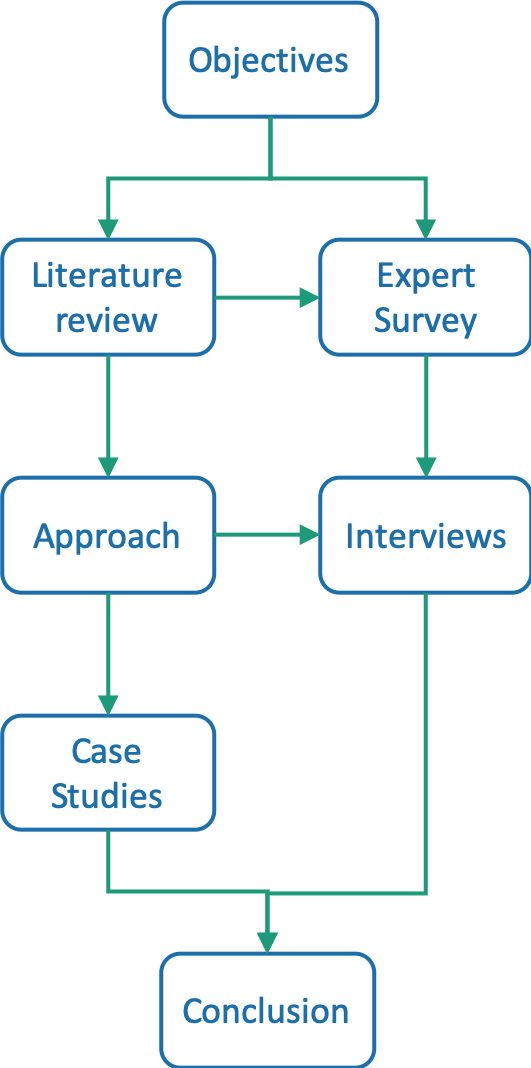
\includegraphics[width=0.5\textwidth]{graphics/thesis-structure}
%\caption{Thesis structure}
%\label{fig:thesis-structure}
%\end{figure}

% introduction
% 
% motivation
% state of the art systems
% system design & architecture
% 
% background, what is system, what features, how does it works
% data processing
% slam and graph minimization
% factor graphs, distance function, graph matching
% trajectory generation
% walking model
% 
% map construction
% observations to map (approximation, regressinon), map to observations (as a sensor)
% (sensor model), propagation model, slam / sam
% 
% conditioning on magnetic field data
% what graphs / figures can be plotted

\begin{description}
    \item[\Autoref{cap:background} - Background]
	The literature review and common concepts of the problem scope.
	Evaluation of current state-of-the-art approaches and technologies.

	\item[\Autoref{cap:TechResearch} - Techonogical research. ]
	Technological roadmap states various possible solutions to human indoor positioning problem. \\
	We develop a model for taking decision of technology / product choice; understanding physical limits. We highlight the landscape of related technologies.
	We use this model for technology choice and for the problem statement.

    \item[\Autoref{cap:thesis_objectives} - Thesis Objectives]
	We define the objectives of our work. Hypotheses we test and a system requirements.

	\item[\Autoref{cap:thesis_methodology} - Methodology]
	Methodology and ideas behind the research. Algorithms and experiments explained.

    \item[\Autoref{cap:conclusion} - Conclusion]
	Conclusion on our results we obtained.


\end{description}



\chapter{Background}
\label{cap:background}
%\epigraphhead[50]{%
%    \epigraph{"if I have seen further it is by standing on the shoulders of Giants."}{Isaac Newton, 1675}
%}

%Here is a comprehensive review of the literature related to the topic of this work.

%We inspired our work from \citet{Chakrabarti2014}.
%\acrshort{sysml} is the reference in this field \citep{ObjectManagementGroup2015}
%The tools keep evolving \citep{Skoltech2017}.

%\todo[inline]{TODO: complete chapter}

%\section{Background and problem statement}
\section{General problem / Introduction / Background
}


\section{Related work}

We review the field of human indoor localization. We focus on crowd-source mapping, or mapping with limited sensor model (limited to existing infrastructure in building space and to sensors in human smartphones).
In this field there are many approaches so solve the sub-problems or parts of given problem. 



For the positioning technologies comparison, we may refer to the paper of \cite{Lymberopoulos} which provides evaluation and comparison of different indoor location technologies and covers the almost most important of them.

While the information about technologies itself is more or less clear. What performance we can reach with given technology? What is the best approach to work with the given technology?

The answer to some questions is simple. The best accuracy is achieved with the biggest database and computational power. But for realistic implementation this is not good enough. The similar approach is to merge all information available in current location and time. The problem again is that how to localize when there is no information available at the current state. The answer is to use the correspondences between previous and future information, to reconstruct the current information. This formulation can be related to the classical SLAM formulation, even if some parts are different.

Different from existing work, we want to re-estimate or post-process all distance and orientations after measurements with information about previous steps are collected. This is called the loop closure process in SLAM literature \cite{orb-slam, orb-slam2}. In fingerprinting literature, there is low number of researches working with re-localization and loop closures. We have to recursively post-process existing data, which has to give us better localization during mapping, and thus better map for future localization.

If magnetic map is not given, the model training can be done by manually collection measurements and marking the locations by special trainers, then the localization model can be generated.

Why magnetic field localization is not a SLAM? SLAM techniques build a map of an unknown environment and localize the sensor in the map with a strong focus on real-time operation \cite{orb-slam}. With magnetic field localization, in every new point we obtain only local information, which is not enough for real-time operation. The difference between camera-based and magnetic fingerprints based localization is significant. Because of this fact, magnetic field localization can’t operate independently in unknown conditions and can’t be considered as SLAM. Nevertheless, we may introduce special aspects of SLAM system to magnetic field localization for better robustness.

The usual camera-based SLAM has the ability to automatically close loops, which means the correction of the accumulated error in exploration after we detect the sensor has returned to a mapped area.

During mapping stage of magnetic field localization, we are constantly accumulating error. \\
We have no tools for error correction because IMU and magnetic field provide both only relative information, and for error correction we need a prior spatial information. \\
The prior information can be collected from other sensors (e.g. beacons, such as WiFi and BLE beacons), information can be human input of location, the prior location can be obtained with camera based place recognition. The most interesting approach is to utilize the information we have in our conditions: previous measurements from magnetic mapping. 

It would be prefect to have loop closure features for robust magnetic field mapping. In practice this is almost never possible. Because of constant growing integration error and small amount of information from magnetic sensor, we have no possibility for conditioning until we mapped the region.

Luckily, conditioning on magnetic field is possible. Once we have a trajectories and observations somehow covering the region, we can try localize on this data. Using the recursive re-localization of existing data we can obtain better solution than initial one.
This part of research is covered in Section \ref{cap:thesis_methodology}.

Why does this even possible to use magnetic field information for localization? The magnetic field in buildings is changing near metal objects, conductive and big structures.
In opposite to traditional idea of compass that is always directed to the north pole, now we have a compass that is slightly deviating.
The idea of localization is that these compass deviations are repetitive in time and space.
Once we reconstructed the magnetic map of the building, we can use these patterns later.

The magnetic field in buildings is changing with time. Even after measurements collected, it is important to update map sequentially. The updates can be done by collecting and processing localization data from all system users. This way we will have the latest data and the system will be more precise.
 
%This approach is called crowdsoursing in related literature. This is why place recognition, map updates and loop closures are the main parts of magnetic field navigation.

An interesting localization system was introduced in Maloc \cite{maloc}: magnetic field based particle filter includes a dynamic step length estimation method. Human step length prediction can be introduced in the localization model, but this is only a part of information possible for given conditions.

Several researches states that the best performance is achieved in multi-sensor or hybrid localization steps. And for walking human localization we may consider a dynamic step length estimation method proposed in \cite{maloc}.

\subsection*{Filtering or global optimization (GraphSLAM)}
We know the paper GraphSLAM based Crowd sourcing framework for indoor Wi-Fi fingerprinting\cite{CrowdsourcingWiFI}. The approach of GraphSLAM is promising. 
%We want to utilize more available spatial information.
The reason for not using GraphSLAM with magnetic fields is only in complexity of system construction. We have to write a gradient descent problem and solve it with GraphSLAM. The problem is that there is no clear gradients in observation model of magnetic field so we can only use filtering methods.

The most promising results in terms of cheap sensor spatial information are magnetic maps. For magnetic fingerprinting there are well developed approaches.

One of well-known papers in magnetic fingerprinting is \cite{Grand20123AxisMF}. The authors present an approach for magnetic field mapping, in terms of not fingerprints, but a full grid mapping procedure. As a result of this mapping procedure we obtain a full filed image that is easy to work with.
The problem with this approach that we have to collect full grid measurements, which is a time consuming procedure. We want to get magnetic field map without additional mapping procedure, this approach is called crowd-source mapping. We collect the data from a set of human travel trajectories. Then we merge them in single noised image (only analogy representation for better understanding), and apply optimization procedure. We require the resulting image be smooth, so the optimization constraints must be set to satisfy the image denoizing procedure. This is just our idea and assumption that is have to be proved in further research.
We see some similarities here with \cite{Cimloc}.

However they are highly dependent(?? prove statement) on the data collection procedure. This algorithms also are not intended for standalone usage in terms of sensors fusion. E.g. requires either special mapping procedures or additional hardware devices - beacons.

There are few papers on magnetic and inertial based navigation. However they were not implemented in SLAM frameworks such as \cite{GraphSLAMCrowdsourceWiFI}. Some of frameworks are a part of commercial interest and are not open source.

The interesting map construction algorithm were proposed in \cite{Cimloc}. 

The full system consists of three subsystems, i.e. Dead Reckoning Subsystem (DRS), Map Construction Subsystem (MCS), and Localization and Navigation Subsystem (LNS). 

Our intuition gives that Dead Reckoning Subsystem performs sensor fusion and smoothing. The localization and navigation subsystem utilities the existing map and the output of smoothed sensors measurements.

The map construction process is an optimization problem with some constraints.

In \cite{Cimloc}, authors propose universal framework with no prior information of building map structure.
But for real situation, the map of the building is known.
We can define an indicator function similar to SLAM occupied cells mapping (????)
With indicator function defined, we may fit the graph of trajectories to the building inner structure graph - topological map.

The similar approach with map constraints correction and re-sampling was shown in \cite{articleXia}. The paper utilizes a   particle   filter that combines PDR and RSSI data.







% motivation
% state of the art systems
% 
\chapter{Technological research}
\label{cap:TechResearch}

This section reports on modern indoor positioning system (IPS) technologies.
There are hundreds of applications for IPS technology. IPS systems are usually based on smartphones (used as a tracking device) and we focus on this application. 
%This usage is the top interest of this paper.
%\begin{abstract}

Objectives:
\begin{itemize}
	\item show the evolution of IPS technology
	\item perform or repeat the research of indoor positioning systems review to compare other IPS publications
	\item visualize IPS usage and work principles (different technologies, connections, FOMs, applications)
	\item create financial and technical models for different IPS technologies
	\item calculate the possible effect of merging different technologies for different applications
	\item calculate in FOMs / prices (novelty)
	\item connect different technologies into single model (where possible)
	\item create system / strategy for optimal* technology choice decision
	\item map / compare existing products and trends over defined figures of mer
\end{itemize}


	% Categories and Subject Description
	% C.3 [Special-purpose and application-based systems]: Realtime and embedded system
	% General Terms
	% Measurement, Performance, Experimentation, Design.

	%/ \subsection{Keywords}
	%Positioning System, Indoor positioning system, Magnetic field, Magnetic fingerprint, Systems for location determination, Wearable computing and innovative mobile devices, IPS, RTLS, GPS mobile-device-based IPS technologies




\subsection{Background / Context}

\cite{Infsoft_wp}

% The market of this technology ...
% Evolution over time.
%
% Enabling technologies
%
% In this paper, we present analysis of indoor positioning techniques.
% IPS is a growing industry with hundreds applications.
%
% Different technologies provide different positive sides and can complement each other.
% The implementation, usage cost and usage scenarios are different for each tech.
%
% different scales of the
% environment.

Indoor navigation solutions is a wide range of products and services. While "indoor routing" functionality that guides people through the buildings is important, there are lots of services which support it, such as content management system, mobile and web applications, indoor and outdoor localization, social networks, data analytics and many others.

Why do we need indoor navigation and positioning? This is because of convenience of global Geo-services, and because of GPS reception problems inside buildings.

One of understandable example of such kind of products is a Google Maps, which are scaled to work inside the buildings.

The situation is much more complicated, the market of indoor positioning is resegmented - different applications from security applications and assets tracking in business and manufacturing to the proximity advertising in retail - from fully protected to broadcast solutions, from cheap high range proximity to high precision solutions in robotics. Indoor positioning systems is a growing industry with hundreds applications.

Different applications have different technologies behind it. Over 15-20 different working technologies is known, about 3-5 of them are widely used now (WiFi, Bluetooth Low Energy, Image Based).

\cite{Infsoft_wp}

% The market of this technology ...
% Evolution over time.
%
% Enabling technologies

In this paper, we present analysis of indoor positioning techniques.

Different technologies provide different positive sides and can be complementary to each other. Combination of complementary technologies can improve the total performance (ultra wide band communication uses a wider range of frequencies and thus have good signal strength and range and allow more precise positioning than single band solutions such as Bluetooth). The implementation process, usage cost and usage scenarios are different for each technologies.

Several technologies are developed to work on a different scales of the environment (local $<$ 1m accuracy, room level $<$ 2m accuracy, floor level 5-10m accuracy, etc.).

For the company developing the products, it is important to consider resources and productiveness. That's why, when we trying to bring product to the market, it's important to create strategy and consider resources we obtain. For this we may use models also.


\subsection{General Objective}


% Current situation on market of IPS, that there are totally different technologies. The IPS products are not very popular, but highly growing.
% understanding trends of technology under this uncertainty is complicated.
%
Indoor navigation is a market solving different problems with logistics inside buildings. The problem is important because more than 90\% of time people usually spend inside the buildings\cite{Indoor_Generation}.

Time spent for logistics such as path choice, search for special places/people can't be measured, but we will agree that it's a wasted time.

Hundreds different applications, dozens of existing technologies, and no really perfect and universal solution. By word perfect we assume comparing to GPS - global, universal, precise enough for usual tasks, stable and free to people.

Existing technologies such as WiFi localization and others will be covered where possible, but the focus of paper is mostly on Indoor positioning as a product it should be: product with price, business plan, technology inside and with the need from customers.

Understanding the technology doesn't bring us to the product.
Indoor positioning applications is a high promising market, which has a lot of uncertainty behind it. First it is a multi-sided and resegmented market, that's why it can't be understood easily. Second, there are many promising technologies in this market which have different behavior. With this level of uncertainty it is important to have information which will allow us to make choice of technology and market segment.

There are several important points in this scientific area to assist in:


-  Taking decision of technology / product choice
-  Understanding physical limits with a feasible model of technology
-  Understand Timeline and Market  scenarios
-  Landscape of technology with literature and patent review


We have to define a strategy and calculate the future effect of applying this technology.
This can be used as a base, for technological investments, product and services development.
Although we can't make the optimal technology choice, the reasonable decision can be taken after mapping existing solutions on a single landscape. Benchmarking, patent and literature research, competitors positioning are also important to define right strategy.

Even knowing the filed in not enough,when we make strategy choice, we have to understand feasibility of this strategy, understand the cost and possible future performance. We can understand technical feasibility of possible future products using system models. In model we want to understand optimal figures of merits for the different possible strategies.

Existing solutions have a high level of complexity. Usually they use a combination of complementary technologies to cover gaps of specific tecnologies. We have to manage the complexity of technical solution with system model if possible. We know that understanding capabilities of each technology and their combination can provide better products and thus important.

\section{Approach}
% 2. Approach (How?) (20%)

First we define current state of the art, we build the model for existing technologies, analyze products on the market, list key players and IP owners, create Pareto frontier. This part is intended to make a visible and understandable landscape of this technology segment.

We use several tools for this: generate artificial intelligence patent classifier with cipher.ai platform, analyze annual market reports and roadmaps from companies \cite{Infsoft_wp}, \cite{trends2019}.

\begin{figure}[ht]
	\centering
	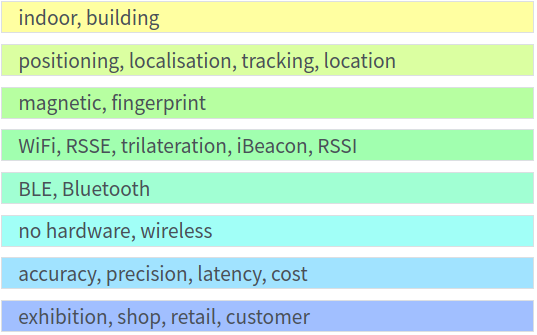
\includegraphics[width=0.48\textwidth]{graphics/roadmap/patents/color.png}
	\caption{Patent keywords search highlighting cipher.ai platform}
	\label{fig:Patent-highlighting}
\end{figure}

Patents search highlighting categories which were used to build the classifier.

\begin{figure}[ht]
	\centering
	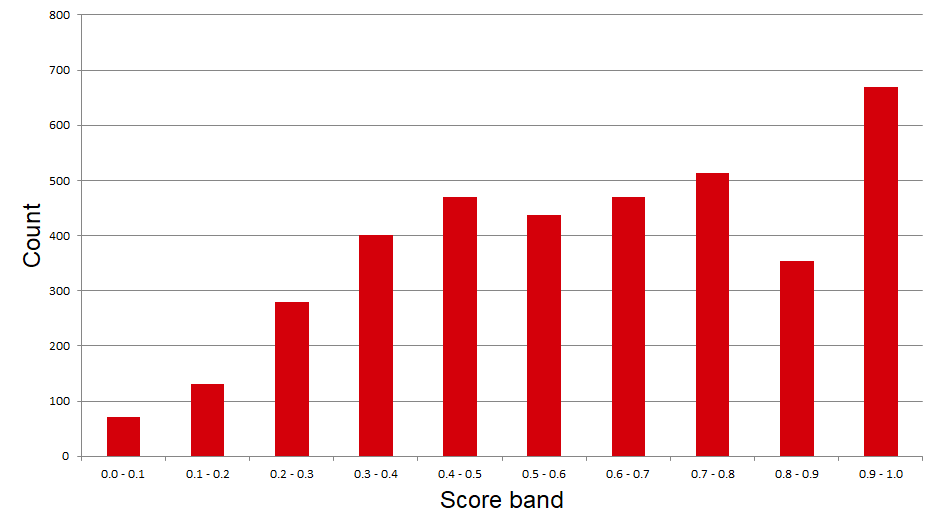
\includegraphics[width=0.65\textwidth]{graphics/roadmap/patents/score.png}
	\caption{Patents result score of final report}
	\label{fig:Patent-score}
\end{figure}

Result score shown on the \ref{fig:Patent-score} show how patents fit the classifier.


Second part is focused on building a model of a product and optimizing it for several criteria.
We focus on the system architecture of indoor positioning solutions. The system architecture provided by the Indoor Location Alliance is used as the main reference. Next we use the data from the Microsoft indoor positioning competition. This is a valuable data, because it provides data about development of indoor positioning technologies and their performance. Data of teams who are competing in the same conditions are perfect for benchmarking. Having the data of benchmarking, we may define technology complexity in real numbers and use it when building the strategy.
% For this we use OPM (object process management) models and OPCAT simulator, UML diagrams, risk matrice and code based models containing figure of merits interconnections. We don't do optimization of a product here, just list possible options with [] curves.

Third we do a financial valuation. We collect all data about product, market, marketing channels and model of sales together.
Having existing business model which is outside of the scope of this paper, we may identify numbers of sales and revenues.
We use the costs and amount of investments we need to complete this project.
We tune the financial model to obtain the positive NPV. To be coherent with the product figures of merits, we also adjust values of the model to receive a non-dominated product on the market.

Next we do value at risk analysis. With the value at risk gain curve, we check different financial models.
% comparing to the Pareto frontier.

After all procedures we come up with bunch of strategies from where we can choose one. Again, we can't make decisions based on this models, but we can check strategies performance and for different technical decisions.

\subsection{Intellectual Property, Publications}

\section{Results}

\subsubsection{Figures of merit}

\setlength{\tabcolsep}{0.5em} % for the horizontal padding
\renewcommand{\arraystretch}{2} % for the vertical padding
\begin{table}[ht!]
%\begin{table*}[]
	\caption{Technology FOM's}
	\label{tab:techFOM}
	\resizebox{\textwidth}{!}{%
		\begin{tabular}{|l|l|L|}
			\hline
			cost hardware, software & USD & cost or hardware rent to provide coverage of needed area with normal operating accuracy \\ \hline
			accuracy & m & accuracy of localization, difference between real position and measurements \\ \hline
			cost & f(USD/sqm) & the cost itself cannot be directly compared because of different types of implementation. Instead, the overall cost presented in several roadmaps is shown. \\ \hline
			range & m & Not important factor, complexity and scalability are affected by this factor. Not representative, because of different types of implementation. Excluded from FOM's \\ \hline
			additional requirements & \begin{tabular}[c]{@{}l@{}}USD;\\ year\end{tabular} & If yes, product is not applicable until they are not solved. Not implemented into model, technologies with additional requirements are mot mapped. (Infrastructure Requirements, Impacts and Notes) \\ \hline
			Scalability & low/med/high & range of scalability, important factor to consider in strategy choice \\ \hline
			Complexity & low/med/high & range of complexity, important factor to consider in strategy choice \\ \hline
			Robustness &  & additional information of what affect the performance of technology \\ \hline
		\end{tabular}%
	}
\end{table}


Lower figures in table are affecting the technology choice, but cannot be added into model, so they are not considered as the figures of merit, but listed in table to explain the reason of excluding them.

\setlength{\tabcolsep}{0.5em} % for the horizontal padding
\renewcommand{\arraystretch}{2} % for the vertical padding
\begin{table}[ht!]
	\caption{Product FOM's}
	\label{tab:ProductFOM}
	\resizebox{\textwidth}{!}{%
		\begin{tabular}{|l|l|l|} \hline
		accuracy & m & accuracy of localization, RMS error between real position and measurements \\ \hline
		development time & month & time to develop the product based on technology with specified accuracy\\  \hline
	\end{tabular}%
	}
	
\end{table}


We focus on the figures of merit which are important for product development, and we use product FOM's mostly\ref{tab:ProductFOM}.


\setlength{\tabcolsep}{0.5em} % for the horizontal padding
\renewcommand{\arraystretch}{2} % for the vertical padding
\begin{table}[ht!]
%\begin{table*}[]
	\caption{Performance of different technologies from the indoor positioning competition}
	\label{tab:my-competition}
	\resizebox{\textwidth}{!}{%
		\begin{tabular}{|l|l|l|l|l|}
			\hline
			Team & Technical Approach & dev.time & RMS error & Team’s Affiliation \\ \hline
			1 & 2.4GHz Phase Offset & 60 & 0.72 & Lambda:4 Entwicklungen \\ \hline
			2 & WiFi+Modulated LEDs & 12 & 2.04 & MSR Asia \\ \hline
			3 & 2.4GHz Time-of-Flight & 72 & 2.03 & Freie Univ. Berlin \\ \hline
			4 & Ultrasonic Time-of-Flight &  & 2.09 & CMU \\ \hline
			5 & IR/Radio Time-of-Flight & 18 & 2.35 & Rutgers \\ \hline
			6 & 2.4GHz Time-of-Flight & 5 & 2.58 & Wroclaw Univ. of Tech. MT-Silesia Sp. \\ \hline
			7 & WiFi+Bluetooth+IMU & 24 & 2.72 & NextoMe \\ \hline
			8 & Modulated Magnetic Signals & 24 & 3.83 & Univ. of Oxford \\ \hline
			9 & SDR Time-of-Flight & 4 & 3.87 & Humboldt Univ. of Berlin \\ \hline
			10 & Modulated Magnetic Signals & 90 & 3.96 & DFKI \\ \hline
			11 & 2.4GHz Phase Offset & 24 & 4.04 & Greina Technologies \\ \hline
			12 & WiFi+Sound Time-of-Flight & 12 & 8.91 & Xian Jiaotong Univ. \\ \hline
			13 & Steerable Antennas ToF & 12 & 10.22 & I.E.C.S. \\ \hline
			14 & Bayesian Filter + WiFi Fingerprinting & 96 & 1.56 & Cork Institute of Technology \\ \hline
			15 & WiFi+IMU Fingerprinting + Neural Network & 36 & 1.96 & Univ. of Cyprus/Cywee \\ \hline
			16 & WiFi Fingerprinting + Neural Network & 12 & 2.22 & Nanyang Tech. Univ. \\ \hline
			17 & WiFi+IMU Fingerprinting & 9 & 2.81 & Ubee S.A. \\ \hline
			18 & WiFi+IMU Fingerprinting + Particle Filter & 24 & 3.19 & MSR Asia \\ \hline
			19 & WiFi Time-of-Flight + Adaptive Filter & 12 & 3.47 & ETH/IMDEA/Armasuisse \\ \hline
			20 & WiFi+IMU+Maps + Conditional Random Fields & 12 & 3.71 & Univ. of Oxford \\ \hline
			21 & WiFi+Magnetic Fingerprinting + Particle Filter & 12 & 4.86 & Nanyang Tech. Univ. \\ \hline
			22 & WiFi+IMU Fingerprinting + Clustering/Decision Trees & 3 & 5.23 & Tata Consulting Services \\ \hline
		\end{tabular}%
	}
\end{table}



Technological limits

3 types: radio (distance), image (angle), fingerprinting (position).

Radio (multilateration, distance measurement), fingerprinting: noise level, wave reflections, sensor errors are main limitations.
Because of noise, the technology limit can’t be reached, only on frequencies where is no external noise, wave reflections - scanning error depends on geometry of signal way.
Image based: accuracy/precision of localisation depends on camera angle resolution. Because trilateration with camera is not possible, error is a linear function of range.



\subsection{State of the art}


\setlength{\tabcolsep}{0.5em} % for the horizontal padding
%\renewcommand{\arraystretch}{2} % for the vertical padding
\begin{table}[ht!]
%\begin{table*}[ht]
	\caption{Technology comparison. Linking grid.}
	\label{tab:linking_grid}
	\resizebox{\textwidth}{!}{%
		\begin{tabular}{lllllllllll|l|l|l|l|l|}
			\cline{12-16}
			&  &  &  &  &  &  &  &  &  &  & \multicolumn{5}{l|}{Products} \\ \cline{12-16}
			&  &  &  &  &  &  &  &  &  &  & \multicolumn{4}{l|}{current} & future \\ \cline{11-16}
			&  &  &  &  &  &  &  &  & \multicolumn{1}{l|}{} & Markets & p1 & p2 & p3 & p4 & p5 \\ \cline{11-16}
			&  &  &  &  &  &  &  & \multicolumn{2}{l}{} & positioning & x & x & x & x & x \\ \cline{11-16}
			&  &  &  &  &  &  &  &  & \multicolumn{1}{l|}{} & marketing & x &  & x &  & x \\ \cline{11-16}
			&  &  &  &  &  &  &  &  & \multicolumn{1}{l|}{} & analytics &  &  & x & x & x \\ \cline{11-16}
			&  &  &  &  &  &  &  &  &  &  &  &  &  &  &  \\ \cline{2-16}
			\multicolumn{1}{l|}{} & \multicolumn{9}{l|}{Technologies} &  &  &  &  &  &  \\ \cline{2-16}
			\multicolumn{1}{l|}{} & \multicolumn{1}{l|}{T1} & \multicolumn{1}{l|}{T2} & \multicolumn{1}{l|}{T3} & \multicolumn{1}{l|}{T4} & \multicolumn{1}{l|}{T5} & \multicolumn{1}{l|}{T6} & \multicolumn{1}{l|}{T7} & \multicolumn{1}{l|}{T8} & \multicolumn{1}{l|}{T9} & Processes &  &  &  &  &  \\ \cline{2-16}
			\multicolumn{1}{l|}{} & \multicolumn{1}{l|}{x} & \multicolumn{1}{l|}{x} & \multicolumn{1}{l|}{x} & \multicolumn{1}{l|}{} & \multicolumn{1}{l|}{} & \multicolumn{1}{l|}{} & \multicolumn{1}{l|}{} & \multicolumn{1}{l|}{x} & \multicolumn{1}{l|}{x} & geofencing &  &  & x &  & x \\ \cline{2-16}
			\multicolumn{1}{l|}{} & \multicolumn{1}{l|}{} & \multicolumn{1}{l|}{} & \multicolumn{1}{l|}{x} & \multicolumn{1}{l|}{x} & \multicolumn{1}{l|}{} & \multicolumn{1}{l|}{x} & \multicolumn{1}{l|}{} & \multicolumn{1}{l|}{} & \multicolumn{1}{l|}{x} & asset tracking &  &  & x & x &  \\ \cline{2-16}
			\multicolumn{1}{l|}{} & \multicolumn{1}{l|}{x} & \multicolumn{1}{l|}{x} & \multicolumn{1}{l|}{x} & \multicolumn{1}{l|}{x} & \multicolumn{1}{l|}{x} & \multicolumn{1}{l|}{} & \multicolumn{1}{l|}{x} & \multicolumn{1}{l|}{x} & \multicolumn{1}{l|}{} & human real-time positioning & x & x & x & x & x \\ \cline{2-16}
			\multicolumn{1}{l|}{} & \multicolumn{1}{l|}{} & \multicolumn{1}{l|}{x} & \multicolumn{1}{l|}{x} & \multicolumn{1}{l|}{x} & \multicolumn{1}{l|}{} & \multicolumn{1}{l|}{} & \multicolumn{1}{l|}{} & \multicolumn{1}{l|}{} & \multicolumn{1}{l|}{} & queue management &  &  & x & x &  \\ \cline{2-16}
			\multicolumn{1}{l|}{} & \multicolumn{1}{l|}{} & \multicolumn{1}{l|}{} & \multicolumn{1}{l|}{x} & \multicolumn{1}{l|}{} & \multicolumn{1}{l|}{x} & \multicolumn{1}{l|}{x} & \multicolumn{1}{l|}{x} & \multicolumn{1}{l|}{} & \multicolumn{1}{l|}{x} & Sensor Fusion SLAM &  &  & x &  &  \\ \cline{2-16}
			\multicolumn{1}{l|}{} & \multicolumn{1}{l|}{x} & \multicolumn{1}{l|}{x} & \multicolumn{1}{l|}{x} & \multicolumn{1}{l|}{x} & \multicolumn{1}{l|}{x} & \multicolumn{1}{l|}{x} & \multicolumn{1}{l|}{x} & \multicolumn{1}{l|}{x} & \multicolumn{1}{l|}{} & map creation & x & x & x & x & x \\ \cline{2-16}
			\multicolumn{1}{l|}{} & \multicolumn{1}{l|}{} & \multicolumn{1}{l|}{} & \multicolumn{1}{l|}{} & \multicolumn{1}{l|}{} & \multicolumn{1}{l|}{} & \multicolumn{1}{l|}{} & \multicolumn{1}{l|}{} & \multicolumn{1}{l|}{} & \multicolumn{1}{l|}{} & Product phase &  &  &  &  &  \\ \hline
			\multicolumn{1}{|l|}{mature} & \multicolumn{1}{l|}{} & \multicolumn{1}{l|}{} & \multicolumn{1}{l|}{} & \multicolumn{1}{l|}{x} & \multicolumn{1}{l|}{} & \multicolumn{1}{l|}{} & \multicolumn{1}{l|}{} & \multicolumn{1}{l|}{} & \multicolumn{1}{l|}{} & Research &  &  & x & x & x \\ \hline
			\multicolumn{1}{|l|}{growth} & \multicolumn{1}{l|}{} & \multicolumn{1}{l|}{} & \multicolumn{1}{l|}{x} & \multicolumn{1}{l|}{} & \multicolumn{1}{l|}{x} & \multicolumn{1}{l|}{x} & \multicolumn{1}{l|}{} & \multicolumn{1}{l|}{x} & \multicolumn{1}{l|}{} & Development & x & x & x & x & x \\ \hline
			\multicolumn{1}{|l|}{emerging} & \multicolumn{1}{l|}{} & \multicolumn{1}{l|}{x} & \multicolumn{1}{l|}{} & \multicolumn{1}{l|}{} & \multicolumn{1}{l|}{} & \multicolumn{1}{l|}{} & \multicolumn{1}{l|}{} & \multicolumn{1}{l|}{} & \multicolumn{1}{l|}{} & Delivery &  &  & x & x &  \\ \hline
			\multicolumn{1}{|l|}{declining} & \multicolumn{1}{l|}{x} & \multicolumn{1}{l|}{} & \multicolumn{1}{l|}{} & \multicolumn{1}{l|}{} & \multicolumn{1}{l|}{} & \multicolumn{1}{l|}{} & \multicolumn{1}{l|}{x} & \multicolumn{1}{l|}{} & \multicolumn{1}{l|}{x} & Support & x & x & x & x &  \\ \hline
		\end{tabular}%
	}
\end{table}



\subsubsection{Positioning}
% companies positioning on market

We have to find products of this companies and other popular products to provide the landscape of market.


Number of patents is a valuable metric but it doesn't show us a value of patent, for example, IndoorAtlas OY obtain patents for magnetic fingerprinting technology which are more valuable now. Some huge companies such as Google LLC and Hitachi are not properly listed. They obtain higher number of patents that shown here, but all of them are not related to indoor navigation, so they are excluded from analysis. Excluding several companies is possible because best products are well known and we want to map products especially.

\cite{Security} It provides information about relative accuracy, mobile device battery usage and other system performance factors to help support early IPS planning and preliminary product evaluation.

\cite{Mautz2012IndoorPT}

IndoorAtlas research of 2016\cite{IPTrise} is a market landscape, which covers most popular technologies, market drivers and future trends. The paper covers adoption and drivers of indoor positioning systems, perspectives of geomagnetic indoor positioning.

Paper \cite{Brena2017} present a comparison of indoor positioning approaches.

% \cite{Kj_fingerprinting, Ashraf_deepnn, Li_geomagnetic, Mautz2012IndoorPT, 8859264, Infsoft_wp}


\setlength{\tabcolsep}{0.5em} % for the horizontal padding
\renewcommand{\arraystretch}{2} % for the vertical padding
\begin{table}[ht!]
%\begin{table}[]
	\caption{Product index}
	\label{tab:productstolink}
	\begin{tabular}{|l|l|}
		\hline
		& Products \\ \hline
		P1 & Mapsted navigation deluxe \\ \hline
		P2 & HERE Indoor Positioning (SDK \& radio mapper) \\ \hline
		P3 & IndoorAtlas \\ \hline
		P4 & VisioGlobe indoor navigation \\ \hline
		P5 & Google VPS (visual positioning system) \\ \hline
	\end{tabular}%
\end{table}


% Please add the following required packages to your document preamble:
% \usepackage{graphicx}
\setlength{\tabcolsep}{0.5em} % for the horizontal padding
\renewcommand{\arraystretch}{2} % for the vertical padding
\begin{table}[ht!]
	\caption{Techologies index}
	\label{tab:techindex}
	\begin{tabular}{|l|l|}
		\hline
		index & sensors \\ \hline
		T1 & GSM / 3G / 4G (LTE) \\ \hline
		T2 & compass, magnetic fields \\ \hline
		T3 & Wi-Fi \\ \hline
		T4 & Bluetooth \\ \hline
		T5 & accelerometer, gyroscope, pedometer \\ \hline
		T6 & UWB antennas \\ \hline
		T7 & Barometer \\ \hline
		T8 & Camera \\ \hline
		T9 & RFID, NFC, QR code \\ \hline
	\end{tabular}%
\end{table}


We use the linking grid to map products \ref{tab:productstolink} to technologies \ref{tab:techindex}. To make table more compact, we use indexes.

\setlength{\tabcolsep}{0.5em} % for the horizontal padding
%\renewcommand{\arraystretch}{2} % for the vertical padding
\begin{table}[ht!]
%\begin{table*}[ht]
	\caption{Technology comparison. Linking grid.}
	\label{tab:linking_grid}
	\resizebox{\textwidth}{!}{%
		\begin{tabular}{lllllllllll|l|l|l|l|l|}
			\cline{12-16}
			&  &  &  &  &  &  &  &  &  &  & \multicolumn{5}{l|}{Products} \\ \cline{12-16}
			&  &  &  &  &  &  &  &  &  &  & \multicolumn{4}{l|}{current} & future \\ \cline{11-16}
			&  &  &  &  &  &  &  &  & \multicolumn{1}{l|}{} & Markets & p1 & p2 & p3 & p4 & p5 \\ \cline{11-16}
			&  &  &  &  &  &  &  & \multicolumn{2}{l}{} & positioning & x & x & x & x & x \\ \cline{11-16}
			&  &  &  &  &  &  &  &  & \multicolumn{1}{l|}{} & marketing & x &  & x &  & x \\ \cline{11-16}
			&  &  &  &  &  &  &  &  & \multicolumn{1}{l|}{} & analytics &  &  & x & x & x \\ \cline{11-16}
			&  &  &  &  &  &  &  &  &  &  &  &  &  &  &  \\ \cline{2-16}
			\multicolumn{1}{l|}{} & \multicolumn{9}{l|}{Technologies} &  &  &  &  &  &  \\ \cline{2-16}
			\multicolumn{1}{l|}{} & \multicolumn{1}{l|}{T1} & \multicolumn{1}{l|}{T2} & \multicolumn{1}{l|}{T3} & \multicolumn{1}{l|}{T4} & \multicolumn{1}{l|}{T5} & \multicolumn{1}{l|}{T6} & \multicolumn{1}{l|}{T7} & \multicolumn{1}{l|}{T8} & \multicolumn{1}{l|}{T9} & Processes &  &  &  &  &  \\ \cline{2-16}
			\multicolumn{1}{l|}{} & \multicolumn{1}{l|}{x} & \multicolumn{1}{l|}{x} & \multicolumn{1}{l|}{x} & \multicolumn{1}{l|}{} & \multicolumn{1}{l|}{} & \multicolumn{1}{l|}{} & \multicolumn{1}{l|}{} & \multicolumn{1}{l|}{x} & \multicolumn{1}{l|}{x} & geofencing &  &  & x &  & x \\ \cline{2-16}
			\multicolumn{1}{l|}{} & \multicolumn{1}{l|}{} & \multicolumn{1}{l|}{} & \multicolumn{1}{l|}{x} & \multicolumn{1}{l|}{x} & \multicolumn{1}{l|}{} & \multicolumn{1}{l|}{x} & \multicolumn{1}{l|}{} & \multicolumn{1}{l|}{} & \multicolumn{1}{l|}{x} & asset tracking &  &  & x & x &  \\ \cline{2-16}
			\multicolumn{1}{l|}{} & \multicolumn{1}{l|}{x} & \multicolumn{1}{l|}{x} & \multicolumn{1}{l|}{x} & \multicolumn{1}{l|}{x} & \multicolumn{1}{l|}{x} & \multicolumn{1}{l|}{} & \multicolumn{1}{l|}{x} & \multicolumn{1}{l|}{x} & \multicolumn{1}{l|}{} & human real-time positioning & x & x & x & x & x \\ \cline{2-16}
			\multicolumn{1}{l|}{} & \multicolumn{1}{l|}{} & \multicolumn{1}{l|}{x} & \multicolumn{1}{l|}{x} & \multicolumn{1}{l|}{x} & \multicolumn{1}{l|}{} & \multicolumn{1}{l|}{} & \multicolumn{1}{l|}{} & \multicolumn{1}{l|}{} & \multicolumn{1}{l|}{} & queue management &  &  & x & x &  \\ \cline{2-16}
			\multicolumn{1}{l|}{} & \multicolumn{1}{l|}{} & \multicolumn{1}{l|}{} & \multicolumn{1}{l|}{x} & \multicolumn{1}{l|}{} & \multicolumn{1}{l|}{x} & \multicolumn{1}{l|}{x} & \multicolumn{1}{l|}{x} & \multicolumn{1}{l|}{} & \multicolumn{1}{l|}{x} & Sensor Fusion SLAM &  &  & x &  &  \\ \cline{2-16}
			\multicolumn{1}{l|}{} & \multicolumn{1}{l|}{x} & \multicolumn{1}{l|}{x} & \multicolumn{1}{l|}{x} & \multicolumn{1}{l|}{x} & \multicolumn{1}{l|}{x} & \multicolumn{1}{l|}{x} & \multicolumn{1}{l|}{x} & \multicolumn{1}{l|}{x} & \multicolumn{1}{l|}{} & map creation & x & x & x & x & x \\ \cline{2-16}
			\multicolumn{1}{l|}{} & \multicolumn{1}{l|}{} & \multicolumn{1}{l|}{} & \multicolumn{1}{l|}{} & \multicolumn{1}{l|}{} & \multicolumn{1}{l|}{} & \multicolumn{1}{l|}{} & \multicolumn{1}{l|}{} & \multicolumn{1}{l|}{} & \multicolumn{1}{l|}{} & Product phase &  &  &  &  &  \\ \hline
			\multicolumn{1}{|l|}{mature} & \multicolumn{1}{l|}{} & \multicolumn{1}{l|}{} & \multicolumn{1}{l|}{} & \multicolumn{1}{l|}{x} & \multicolumn{1}{l|}{} & \multicolumn{1}{l|}{} & \multicolumn{1}{l|}{} & \multicolumn{1}{l|}{} & \multicolumn{1}{l|}{} & Research &  &  & x & x & x \\ \hline
			\multicolumn{1}{|l|}{growth} & \multicolumn{1}{l|}{} & \multicolumn{1}{l|}{} & \multicolumn{1}{l|}{x} & \multicolumn{1}{l|}{} & \multicolumn{1}{l|}{x} & \multicolumn{1}{l|}{x} & \multicolumn{1}{l|}{} & \multicolumn{1}{l|}{x} & \multicolumn{1}{l|}{} & Development & x & x & x & x & x \\ \hline
			\multicolumn{1}{|l|}{emerging} & \multicolumn{1}{l|}{} & \multicolumn{1}{l|}{x} & \multicolumn{1}{l|}{} & \multicolumn{1}{l|}{} & \multicolumn{1}{l|}{} & \multicolumn{1}{l|}{} & \multicolumn{1}{l|}{} & \multicolumn{1}{l|}{} & \multicolumn{1}{l|}{} & Delivery &  &  & x & x &  \\ \hline
			\multicolumn{1}{|l|}{declining} & \multicolumn{1}{l|}{x} & \multicolumn{1}{l|}{} & \multicolumn{1}{l|}{} & \multicolumn{1}{l|}{} & \multicolumn{1}{l|}{} & \multicolumn{1}{l|}{} & \multicolumn{1}{l|}{x} & \multicolumn{1}{l|}{} & \multicolumn{1}{l|}{x} & Support & x & x & x & x &  \\ \hline
		\end{tabular}%
	}
\end{table}


In linking grid \ref{tab:linking_grid}, we map technologies to possible processes in indoor positioning systems. For each technology, we identify the technology adoption or readiness level in simplest form. After that, for each process, we mark all possible technologies involved. Then we mark products to markets and identify which processes are involved into each product, on which markets the product is positioned and what the level of this product on the market.


\subsubsection{Patents}

\begin{figure}[ht]
	\centering
	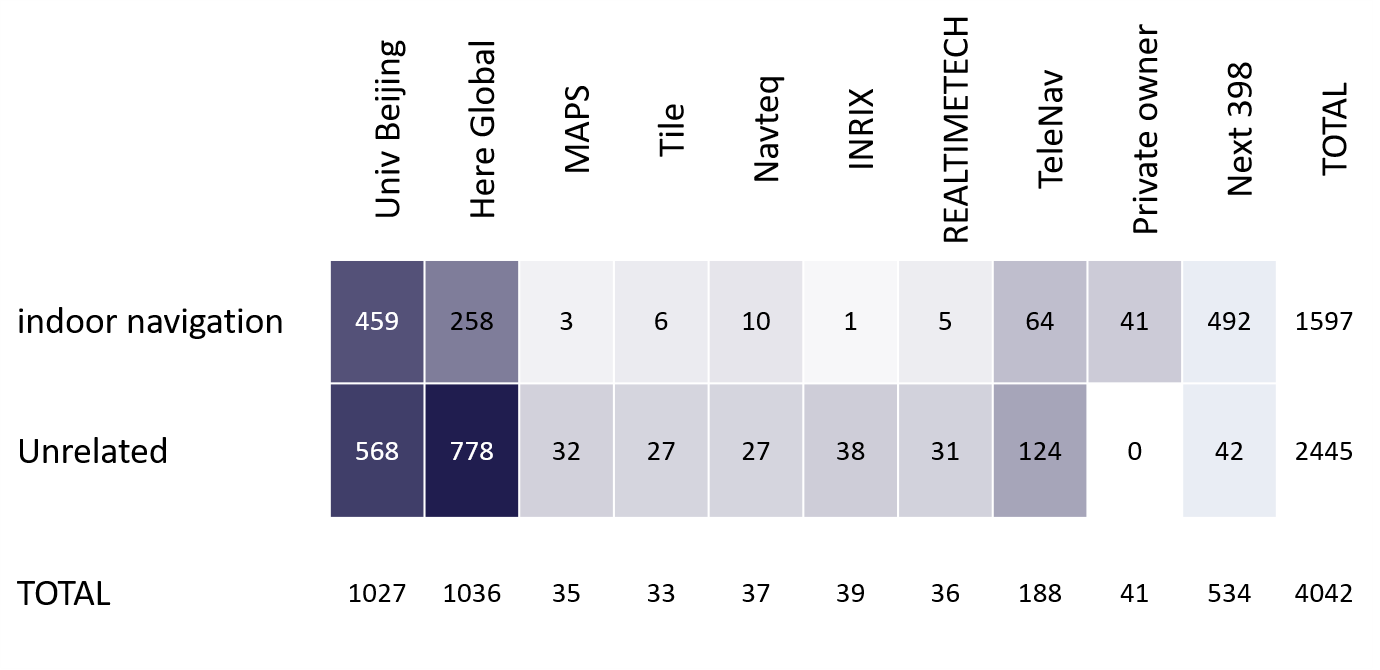
\includegraphics[width=0.7\textwidth]{graphics/roadmap/patents/Patenting2.png}
	\caption{Portfolio size: Active patent families, by organization and technology. Currently active patent families (granted or pending) by organization and technology.}
	\label{fig:Patent-families2}
\end{figure}

In patent research of current field, we use patent classifier with the training set of 590 positive and 136 negative patents marked.
Using this classifier and AI patent platform cipher.ai, we do the organization search which is presented on \ref{fig:Patent-families2}
. On the Figure \ref{fig:Patent-families2} category of "Unrelated" is the category of patents that does not fit the classifier.


\begin{figure*}[ht]
	\centering
	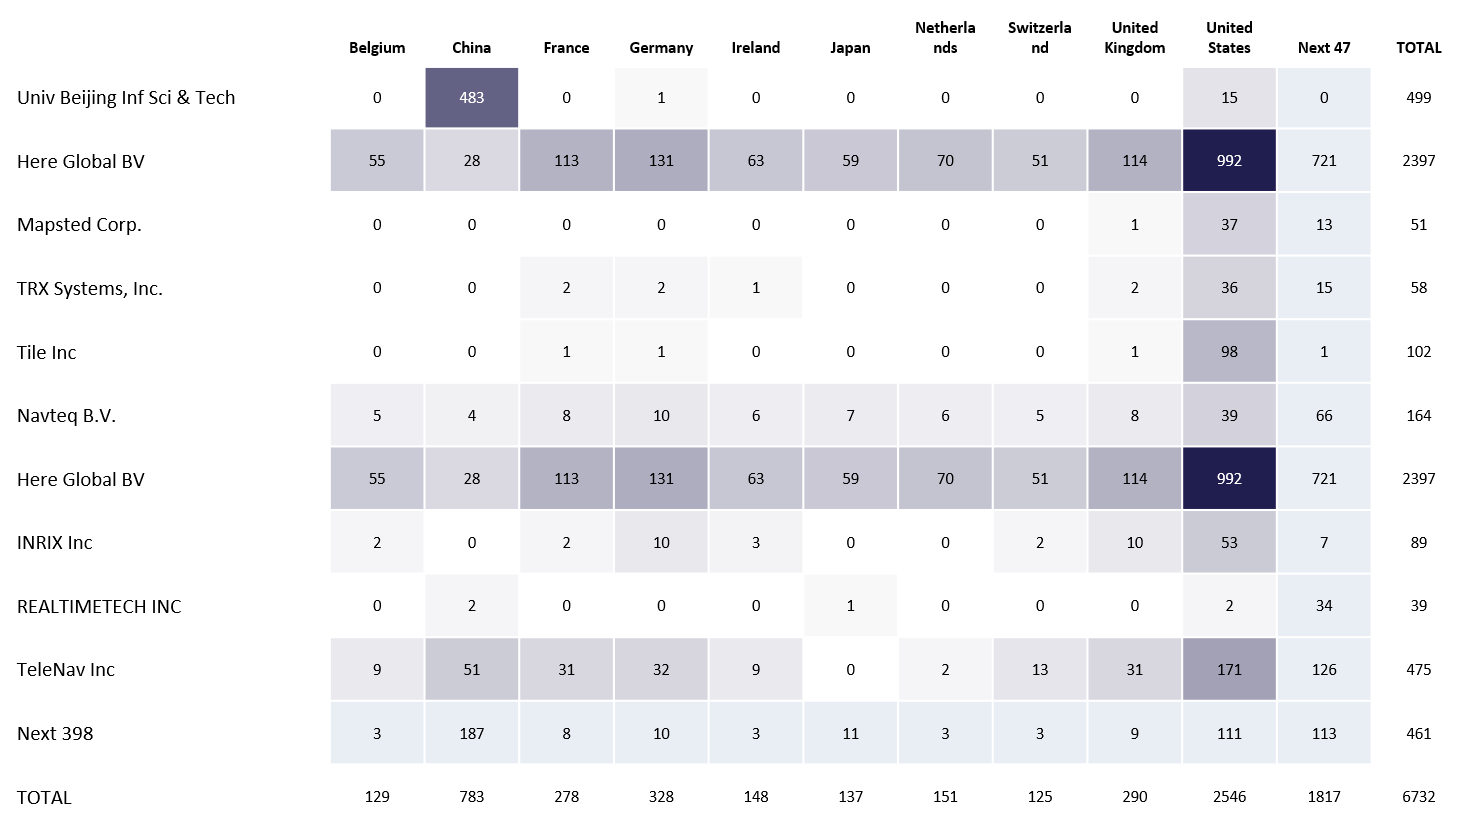
\includegraphics[width=\textwidth]{graphics/roadmap/patents/Geography Granted patents by country and organisation.png}
	\caption{Geography: Granted patents, by country and organization
		Currently active and granted individual patents per country, by organization.}
	\label{fig:Granted-patents-by-coutry}
\end{figure*}

\setlength{\tabcolsep}{0.5em} % for the horizontal padding
%\renewcommand{\arraystretch}{2} % for the vertical padding
\begin{table}[ht!]
%\begin{table*}[]
	\caption{Portfolio size: Active patent families, by organization and technology}
	\label{tab:patents-scope}
	\resizebox{\textwidth}{!}{%
		\begin{tabular}{lllllllllll}
			& Univ Beijing & Here Global & MAPS & Tile & Navteq & REALTIMETECH & TeleNav & Private owner & Next 398 & TOTAL \\
			indoor navigation & 459 & 258 & 3 & 6 & 10 & 5 & 64 & 41 & 492 & 1597 \\
			Unrelated & 568 & 778 & 32 & 27 & 27 & 31 & 124 & 0 & 42 & 2445 \\
			TOTAL & 1027 & 1036 & 35 & 33 & 37 & 36 & 188 & 41 & 534 & 4042
		\end{tabular}%
	}
\end{table}


\setlength{\tabcolsep}{0.5em} % for the horizontal padding
%\renewcommand{\arraystretch}{2} % for the vertical padding
\begin{table}[ht!]
%\begin{table*}[]
	\caption{Geography: Granted patents, by country and organization}
	\label{tab:patents-map}
	\resizebox{\textwidth}{!}{%
		\begin{tabular}{lllllllllllll}
			& Belgium & China & France & Germany & Ireland & Japan & Netherlands & Switzerland & United Kingdom & United States & Next 47 & TOTAL \\
			Univ Beijing Inf Sci \& Tech & 0 & 483 & 0 & 1 & 0 & 0 & 0 & 0 & 0 & 15 & 0 & 499 \\
			Here Global BV & 55 & 28 & 113 & 131 & 63 & 59 & 70 & 51 & 114 & 992 & 721 & 2397 \\
			Mapsted Corp. & 0 & 0 & 0 & 0 & 0 & 0 & 0 & 0 & 1 & 37 & 13 & 51 \\
			TRX Systems, Inc. & 0 & 0 & 2 & 2 & 1 & 0 & 0 & 0 & 2 & 36 & 15 & 58 \\
			Tile Inc & 0 & 0 & 1 & 1 & 0 & 0 & 0 & 0 & 1 & 98 & 1 & 102 \\
			Navteq B.V. & 5 & 4 & 8 & 10 & 6 & 7 & 6 & 5 & 8 & 39 & 66 & 164 \\
			Here Global BV & 55 & 28 & 113 & 131 & 63 & 59 & 70 & 51 & 114 & 992 & 721 & 2397 \\
			INRIX Inc & 2 & 0 & 2 & 10 & 3 & 0 & 0 & 2 & 10 & 53 & 7 & 89 \\
			REALTIMETECH INC & 0 & 2 & 0 & 0 & 0 & 1 & 0 & 0 & 0 & 2 & 34 & 39 \\
			TeleNav Inc & 9 & 51 & 31 & 32 & 9 & 0 & 2 & 13 & 31 & 171 & 126 & 475 \\
			Next 398 & 3 & 187 & 8 & 10 & 3 & 11 & 3 & 3 & 9 & 111 & 113 & 461 \\
			TOTAL & 129 & 783 & 278 & 328 & 148 & 137 & 151 & 125 & 290 & 2546 & 1817 & 6732
		\end{tabular}%
	}
\end{table}


\subsection{Building a model}

% What points are we roadmap?

% usage of technology
% possible applications

\subsubsection{Architecture}

One way of AI usage with indoor positioning system is shown in post of IBM-research group \cite{AI-Centric_IPS}. This gives us some view of architecture and data transactions in modern IPS applications.

\begin{figure}[ht]
	\centering
	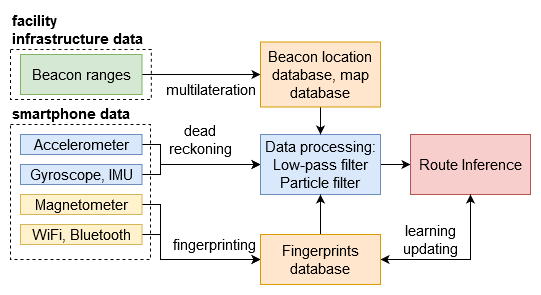
\includegraphics[width=0.65\textwidth]{graphics/roadmap/indoor navigation roadmap-Page-3.png}
	\caption{Signal processing system architecture}
	\label{fig:arch}
\end{figure}

On figure \ref{fig:arch} we present possible architecture of indoor positioning application.
We use blue colour for dead-reckoning application. Because of different smartphone sensors, signal processing will be different for every smartphone model, that's why signal processing should be done on the smartphone itself.

After first signal filtering from inertial and others complementary sensors (barometer), all information from sensors has to be matched with fingerprint database and map databases. This process can be done on the remote server or locally, this depends on system architecture chosen.

The technology choice of system architecture can't be explained, because there is no single strategy for system design.

Only several assumptions can be presented:

\begin{itemize}
	\item Server based systems can be provided by an external vendor - buying a service
	\item Server based systems are enough cost effective to be used (development of server platforms in 2020 is enough to not care about signal processing on the local devices)
	\item Mobile device based are harder in development and support
	\item Mobile device based systems may not require external server and can be run locally - stable work with no internet connection
	\item Once operating, mobile device based are cheaper, because no server support and rent needed - costs are on user side. Important for scalability (if one million of users will use system, some additional traffic management will be required)
	\item Emergency help services shall not depend on internet connection - broadcast systems, mobile device used as transmitter - mobile device initiated systems
	\item In some cases network initiated positioning can be useful. For example, if ultrasound waves are used for positioning, sound transmission will happen over short periods of time defined by network, this will reduce level of noise.
\end{itemize}

For the most common case of human tracking with no special requirements on internet connection, scalability and sensors used, architecture shown of \ref{fig:arch} can be used.

\begin{figure}[ht]
	\centering
	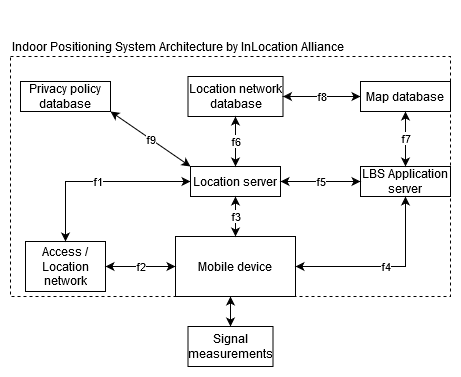
\includegraphics[width=0.6\textwidth]{graphics/roadmap/InLocation Alliance (ILA).png}
	\caption{InLocation Alliance (ILA) system architecture}
	\label{fig:arch2}
\end{figure}

InLocation Alliance (ILA) was founded in 2012 and worked on indoor positioning solutions. In 2014 the ILA created an open, technology-independent architecture in support of accurate location of mobile devices within different types of indoor venues (see Figure \ref{fig:arch2}), which presents seven key system elements and nine interfaces.

What we see from Figure \ref{fig:arch2}, is that only mobile devices are considered as input, current architecture don't have beacons in it.

Results of ILA work and standards they make are not open and published, so they are not a standard now and we may freely update this structure.
Moreover, in \cite{Security} author propose to define both system architecture diagrams \ref{fig:arch} and \ref{fig:arch2} and use them as a product documentation to describe interfaces and so on.

% The ILA System Architecture (SA) specifies the main components and interface requirements of a technology-independent system architecture for indoor location.

% The SA has been designed to support a wide range of venues: from the very small (e.g. stand-alone business) to the very large (e.g. corporate campus) to the very distributed (e.g. worldwide retail chain).
% The SA is based on open interfaces in order to support multi-vendor environments for indoor location.
% While the SA in itself is generic and technology agnostic, the focus of the first public release of the SA is on Wi-Fi and BT.

\subsubsection{Roadmap system modelling}
% \subsubsection{Roadmap model in OPM}

From \cite{Security}, the process of documenting architecture can be described as:

At the appropriate times, take steps with prospective system providers:
\begin{itemize}
	\item Provide the two architecture diagrams to prospective vendors
	\item Ask vendors to document the architecture and positioning mode(s) of the IPS being considered, relative to these architecture diagrams.
	\item Plan and document any data import or export functions.
	\item Review the existing system’s reporting capabilities against \ what reporting requirements apply for business uses of the system.
	\item Review what applications reside where, such as an on-premises server or a cloud server.
\end{itemize}

We will create an OPM model using this approach and Figures \ref{fig:arch} and \ref{fig:arch2}.

\begin{figure*}[ht]
	\centering
	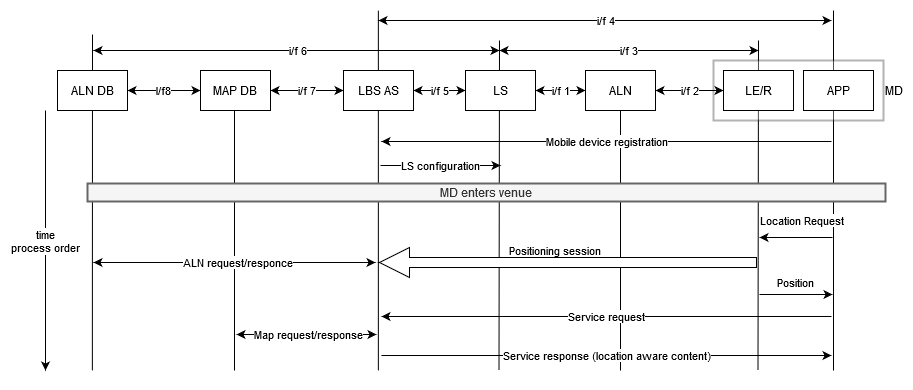
\includegraphics[width=\textwidth]{graphics/roadmap/location aware content by ILA.png}
	\caption{Location aware content example by ILA.}
	\label{fig:loc_aware}
\end{figure*}

We present an example from \cite{ILA-System-Architecture} of how location aware content is delivered to users.
On Figure \ref{fig:loc_aware}, we see the order of steps, used to provide location aware content to user, e.g. geo-targeting or geo-fencing. This diagram doesn't explain much the structure and interfaces of system architecture, but shows some connections between them. All short naming are the same as in Figure \ref{fig:arch2}.

% For better structure representation we will use OPM models.



\subsection{Technology Strategy Vision}

% explain vision and strategy

From annual reports\cite{trends2017,trends2019} we can get history of trends in mobile marketing. When and where it is possible,different technologies and services are implemented in IPS. We will list several trends of indoor positioning systems.


Merge of indoor and outdoor positioning systems:
It is visible that IPS technologies are converging to some set of technologies. When this will happen, the connection between IPS and GPS or other outdoor positioning systems can be done. Right now, several IPS products support this feature, but this is not a global solution.\cite{Brena2017}
Privacy and security in IPS development:
Current trends with protection of users in web (GDPR policies) bring us to the point that some steps in this direction are done by government. Development of a product which is privacy safe can improve the adoption of use, which is important factor now. This factor directly affects the scalability of specific technologies and products.\cite{Brena2017}
Crowd-source mapping:
Most of technologies used in IPS systems requires hours of measurements inside the facilities to create a map of a building. Regular users can provide big amount of measurements, needed to create map of building and update it regularly.  This approach is important for applications that don't require special equipment for measurements and need regular map update (magnetic fields, WiFi, ambient sound localization technologies).\cite{Brena2017}
"China Crisis Ebbs, But Tracking Apps Are Going Strong" - the article of today's paper in The New York Times \cite{Tracking_Apps_times}.
Having the great need of tracking people, new products of human tracking were developed rapidly. "But the authorities have set few limits on how that data can be used. And now,officials in some places are loading their apps with new features, hoping the software will live on as more than just an emergency measure."
Indoor Location of E911 Mobile Callers:
Enhanced 911 Services enable 911 operators to:
Immediately pinpoint the location of the 911 caller based on the calling number
Callback the 911 caller if a disconnect occurs
Tracking location of people in emergency situation is an important challenge and one of the most important drivers of current IPS technology.
The initiative shown some results in 2013, but USA government requires universal service that will be implemented across the USA. One of the key points of this measure, that it has to work indoors. Importance of E911 point is that several actions are already done and several technological steps may change the state of USA market which may happen in future 2-5 years.

The overall strategy is to deliver the product in least development time, while reaching the average accuracy.

\subsection{Timeline}

We use data of Microsoft competition as a starting reference. In table \ref{tab:my-competition}, we have time of development and resulting accuracy for the different technology choice of different teams participated.
We may use these dependencies to understand, what time is needed to achieve each level of accuracy for different combinations of technologies.

\begin{figure}
	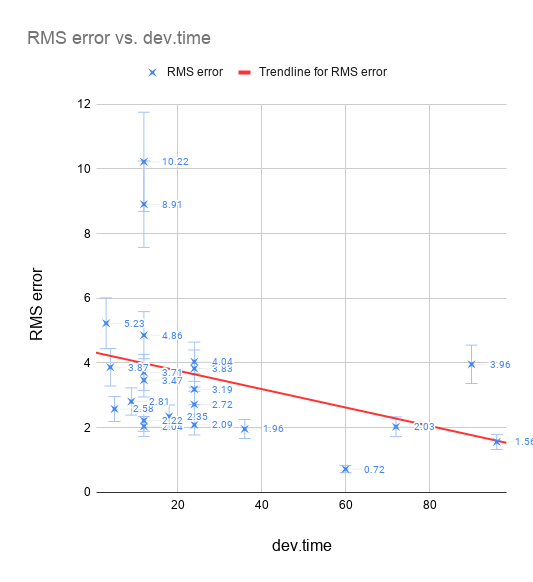
\includegraphics[width=0.6\textwidth]{graphics/roadmap/RMSerrorvsdevtime.png}
	\caption{Root mean square error of positioning versus time of development}
	\label{im:rmse}
\end{figure}

On figure \ref{im:rmse}, we see the team competitors performance versus time for development in months.

\begin{table}[]
	\caption{Technology choice.}
	\label{tab:best-tech}
	\begin{tabular}{lll}
		Technical Approach & dev.time & RMS error \\
		SDR Time-of-Flight & 4 & 3.87 \\
		2.4GHz Time-of-Flight & 5 & 2.58 \\
		WiFi+IMU Fingerprinting & 9 & 2.81 \\
		WiFi+Modulated LEDs & 12 & 2.04 \\
		WiFi Fingerprinting + Neural Network & 12 & 2.22 \\
		WiFi+IMU Fingerprinting + Neural Network & 36 & 1.96 \\
		2.4GHz Phase Offset & 60 & 0.72 \\
		Bayesian Filter + WiFi Fingerprinting & 96 & 1.56
	\end{tabular}%
\end{table}

We choose the best performance in technologies \ref{tab:best-tech} by multiplication of all of parameters.
We define the metric as:
\begin{equation*}
	\textsf{performance} = \frac{1}{\textsf{(development time)} \cdot \textsf{accuracy}}
\end{equation*}

We predict the accuracy of or product in between of optimal scenario (non-dominated points) and the trend line. From this we may present a timeline.

\begin{figure*}[t]
	\centering
	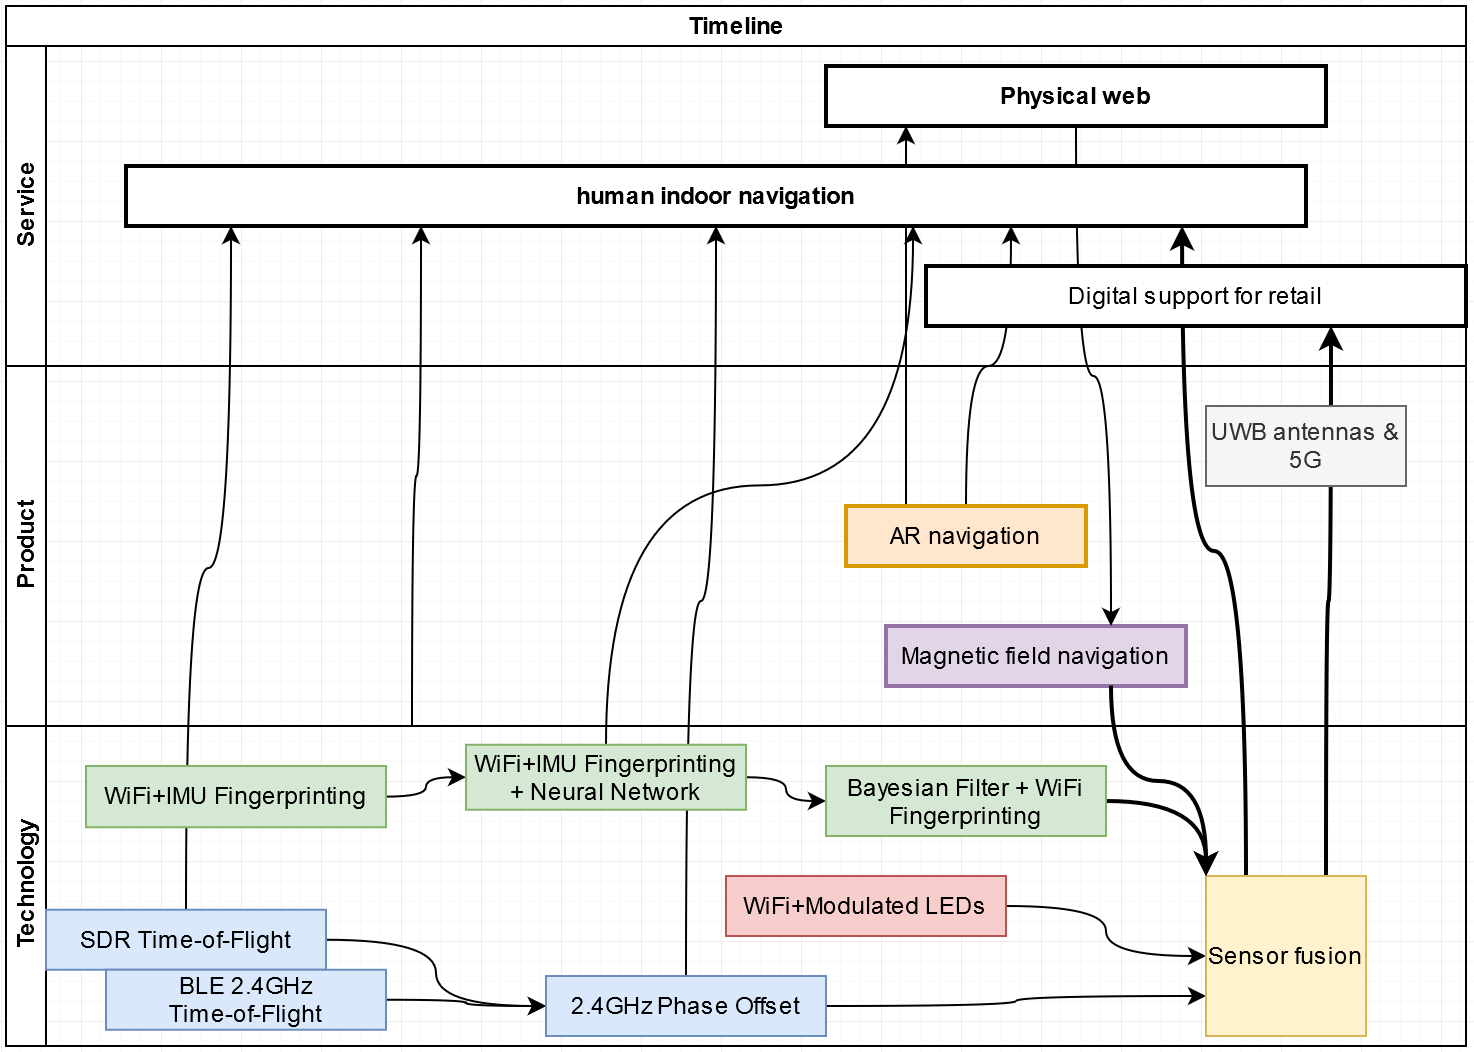
\includegraphics[width=0.99\textwidth]{graphics/roadmap/timeline.png}
	\caption{Timeline diagram. Left to right: Passed term, Short term (1-2 years), Long term (2-5 years).}
	\label{fig:timeline}
\end{figure*}

On \ref{fig:timeline} we show the action plan for development the product with different alternative strategies.
% historical evolution of trends in mobile technologies and technologies of indoor positioning.

The overall trend is that IPS products are converging to a global ecosystem - digitization of cities. After human and assets will be tracked constantly, this will be a big supplementation to a smart cities technologies.
Before that, there is the market of IPS in retail applications (asset tracking, geofencing, way finding, proximity marketing)\cite{Infsoft_wp}.

By speaking of current situation on the market, we can say that human indoor tracking is growing, but it is not mature.
We are building product with the main function of human indoor positioning as shown on Figure\ref{fig:timeline}.

Magnetic field navigation is another perspective factor in the timeline, some progress is already achieved by IndoorAtlas company in this field, but this technology will might become global and will assist the usual dead reckoning and existing WiFi and BLE technologies.

UWB localization can be better than existing radio-based technologies, but until there is no UWB communication equipment in smartphones and facilities worldwide. Spreading of 5G may change this situation.
%
% The matchmaking apps are stated in the timeline, because it is the interest of current paper product research. This is the way of usage the IPS technology which merges social networks and geo-based services.
% \begin{wrapfigure}{l}{0.7\linewidth}
% 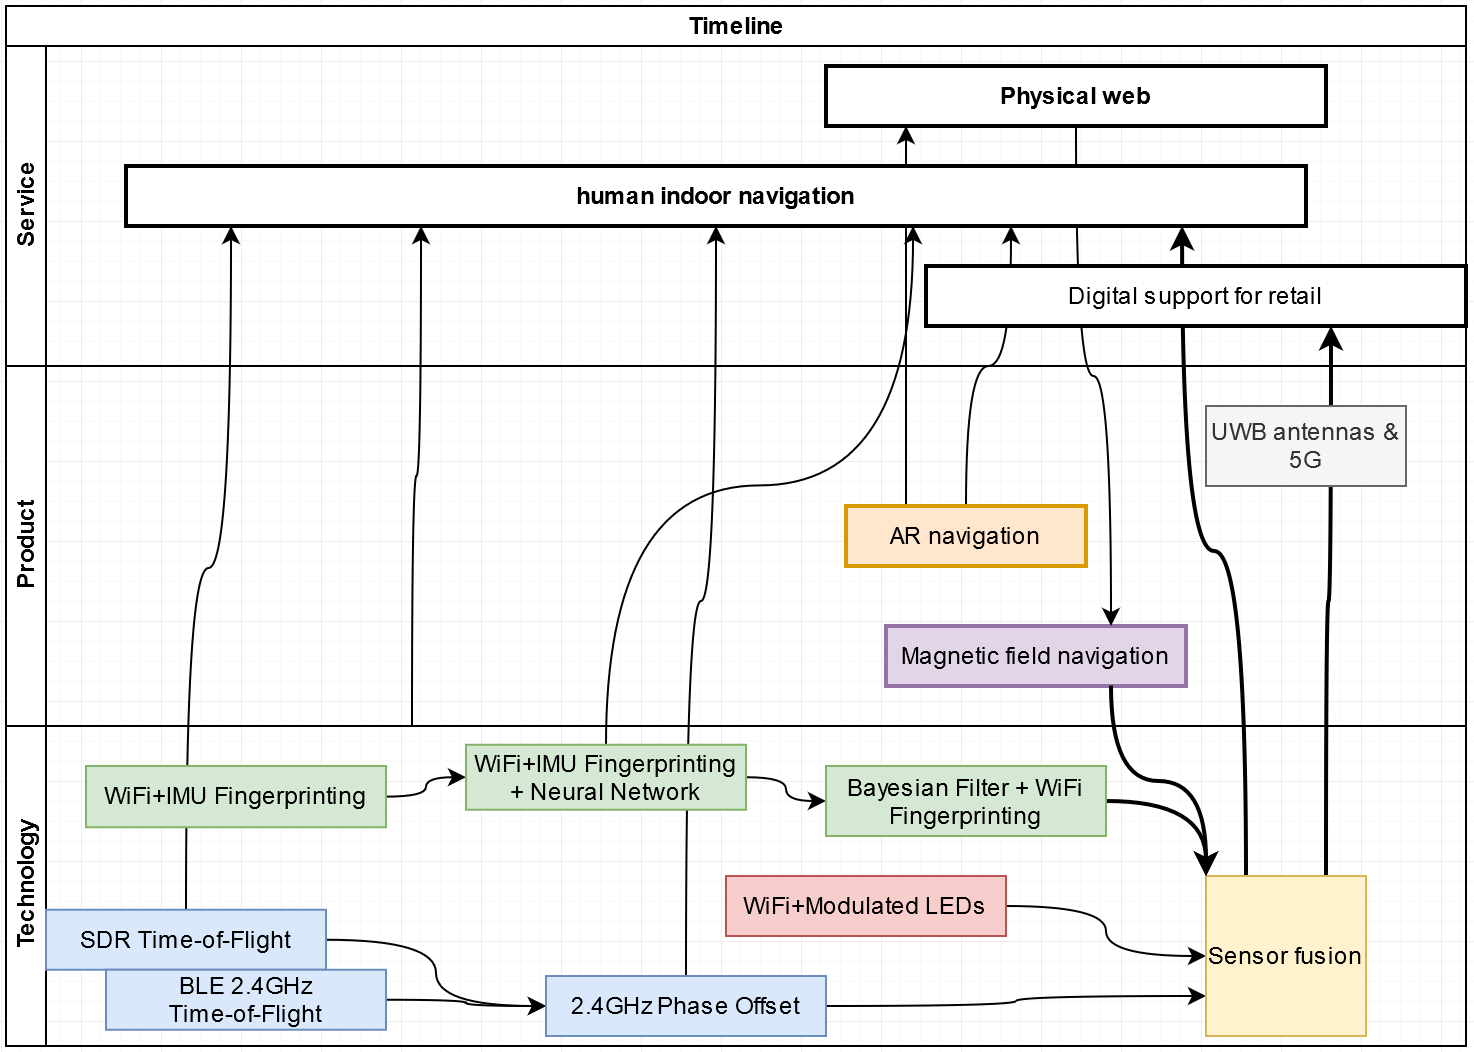
\includegraphics[width=\linewidth]{graphics/roadmap/timeline.png}
% \caption{This is the former Share\LaTeX{} logo}
% \end{wrapfigure}
% To present current landscape, we will state known trends of this field.
% Because of uncertainty behind this information, in timeline they all can be marked under "Future applications".

\subsection{Technical feasibility}

Physical limits of indoor positioning system come from the environment. Real usage limits are more flexible and are directed by human limits (reaction time).

Applicable limits of each of FOM-s are different for different applications. For people to navigate, the accuracy of (1 m) and response frequency of (5 s)  may be enough. In big environment, the accuracy of 1-3 meters (similar to GPS performance) is enough. For the high performance applications, the accuracy must be lower than 1m (0.1 -0.5)m and response frequency near (0.1-0.5)s. In ARkit research[1] proposed model, where accuracy required is equal to 10 percent of the distance between various points of the destination, which gives us same 0.4-0.5m for rooms and 4-5m for big halls.


The range for RSSI method is calculated by formula:

$\mathbf{ dist = 10 * ((RSSI_{1m} - RSSI_{rec})/(10 * Path loss)) }$

Main limitation with this type of distance calculation is sensor's sensitivity and field noise. Having -96 DBm sensitivity and 4 DBm transmit power, system will be operable in range of 30m.

\begin{figure}
	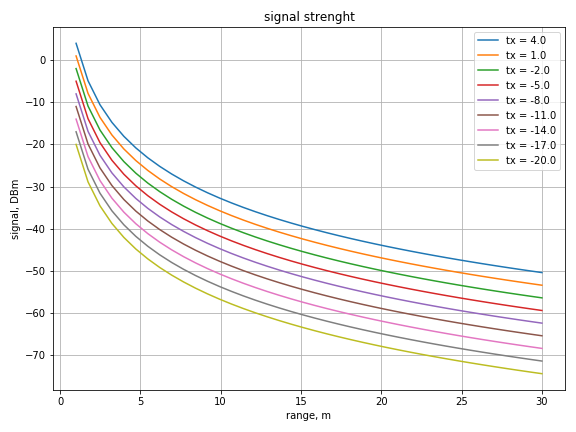
\includegraphics[width=0.49\textwidth]{graphics/roadmap/signal_strenght.png}
	\caption{Radio signal strength distribution model.}
	\label{fig:signal}
\end{figure}
To calculate the signal distribution, we use Free-space path loss formula and Log-distance path loss model.

We use constants from signal measurements in [21], and Log-distance path loss model.

This gives us the information that signal transmission quality depends of distance, transmitter power and receiver sensitivity.

For BLE, we the normal conditions are as in figure above: with normal operating range of 30m, transmitter power in [4 DBm, -20 DBm] range, receiver sensitivity in range of -40 DBm, -60 DBm.

The limits for tracking technologies are not strict, they are only affecting accuracy and precision of localization. We can use table of normal ranges for technologies as a reference, but the performance will depend of huge amount of factors which can't be modeled accurately.

\subsection{Financial Valuation}

\begin{align}
\textsf{Customer Acquisition Cost (CAC)} &= \frac{\textsf{(product cost) + sales + marketing}}{\textsf{(number of customers)}}  \\
\textsf{Life-Time Value (LTV)} &= \textsf{(average value of sales)} \times \textsf{(number of repeat transactions)} \times \notag\\
&\times \textsf{(average retention time)} \\
\textsf{Profit} &= \textsf{LTV} \times\textsf{(average margin)}
\end{align}


Assumptions:

\begin{enumerate}
	\item     an exhibition area of 1000 sqm, needs 9 BLE anchors for full coverage
	\item     Calculations for 1 day
	\item     1000 visitors per day
	\item     Mobile app development needs 4hrs of programming
	\item     1 person for hardware installation and removal
\end{enumerate}

Assumptions on revenues rate are shown on the figure above.

Plan A:

CAC~a~ to charge each booth (participating company) to benefit from indoor navigation facilities per day

Daily costs of operation = 1200 USD; Fixed costs = 3000 USD;

Plan B:

CAC~B~to charge each booth (participating company) to benefit from indoor navigation facilities + additional product features

Daily costs of operation = 1700 USD; Fixed costs = 2000 USD;

\begin{figure}
	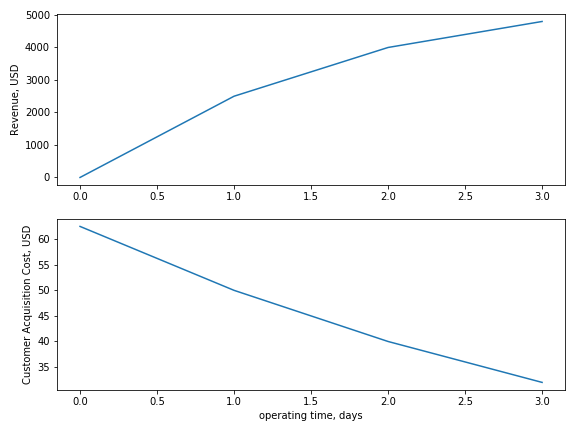
\includegraphics[width=0.49\textwidth]{graphics/roadmap/fin/varg_10runs.png}
	\caption{Customer acquisition cost}
	\label{fig:cac}
\end{figure}

We assume that in strategies, CAC is different, and costs are different. Number of customers is assumed probabilistic as a triangular distribution. We use the assumption in the model, that for the longer operation time, customers get a discount as a power function of power 0.8.

The total revenue and customer acquisition cost are presented on the Figure \ref{fig:cac}. This is an example for one strategy, average customer acquisition is about 45 USD per day. Average revenue is about 1800 USD per day.

%We are modelling two strategies for operating time of 2 and 5 days.
%Watching on the figure, we understand that strategy A is better on a short term, and on a long operating time, both strategies are almost equal.


\begin{figure}
	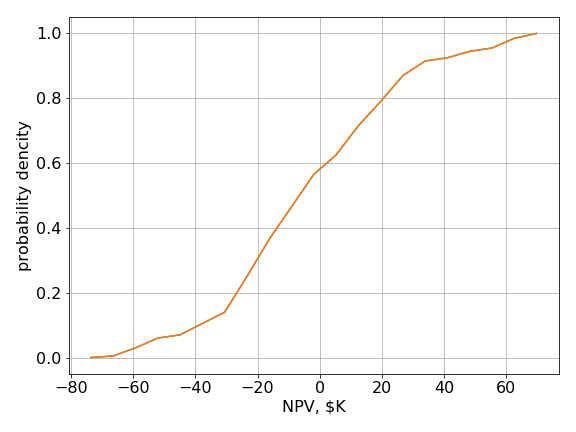
\includegraphics[width=0.49\textwidth]{graphics/roadmap/fin/varg_mruns.png}
	\caption{Value at risk gain curve}
	\label{fig:varg}
\end{figure}

\section{Validation}


The tech background is validated by comparison of scientific publications \cite{ILA-System-Architecture}, \cite{Brena2017, Kj_fingerprinting, Li_geomagnetic, Mautz2012IndoorPT, AI-Centric_IPS} and analysis of the existing solutions.
The business model was sequentially developed to satisfy four fits model.
Expert validation (IndoorAtlas expert's interview, customer's interview).

One of the most valuable tools for the roadmap developing was benchmarking with existing researches \cite{microsoft}.

\section{Conclusions}
% 5. Conclusions & Lessons Learnt from TPR:F/TPR:A (10%)

The indoor navigation product strategy tool is in development now.
It was proven to be viable by customer discovery process and by revenue model \& calculation.

However, in order use this tool efficiently, this strategy tool requires:
\begin{enumerate}
	\item to be accurate - proved to be possible but requires lot of engineering
	\item to be convenient - depends on the way of realization and would require continuous improvements
	\item acceptance of the market segment, which shall be accurately chosen
	\item complexity of either software or hardware
\end{enumerate}

This paper shows the usage of different modelling approaches, which allows to develop the strategy based on the product model.

Paper provides a roadmap, technology landscape and technology strategy choice that is based on the timeline and all relevant roadmap elements.
Each statement is supported by a quantitative fact or analytics defined by the models of product and technology.

System model, created in this paper, list all important figures, components and capabilities. The key functions and system architecture are identified using common standards. Figures of merit identify capabilities and limits of technology and provide information about product development strategy. The demonstrators, patents, known products and products which can be used as a components of indoor positioning system are listed in paper and implemented into strategy.

In paper, we identify the limit for the product development performance as an average performance (root mean square trend line). This allow us to make a strategy choice, to develop a product/technology or to buy it.

The financial valuation was developed, based on product model and sales models.
We use probabilistic models to develop strategy under uncertainty. Different scenarios (pessimistic, baseline, optimistic) are defined.

% Taking decision of technology / product choice - Understanding physical limits. Highlighting the landscape of related technologies.

% system design & architecture
% 
\chapter{Thesis Objectives}
\label{cap:thesis_objectives}


In this chapter we define the goals and derive the specific questions to be addressed in our research.

%\section{Objectives}
We perform this research to create an indoor positioning system with special features. The objective of this research is to develop all algorithms needed to obtain these features.

We define an approach for dealing with the dead reckoning system. We propose a mapping algorithm using ARcore visual odometry for training and all-time pedestrian dead reckoning and magnetic mapping for operation.

We aim to develop the system, working without complicated sensors or physical landmarks as beacons. This is only a research interest because the current SOTA PDR systems are only secondary to other approaches.

%The problem we solve and the scope can be formulated as the following: 
We design the algorithm of data collection and for the purpose of mapping indoor location and localization usage. 
We evaluate algorithm's robustness, by means that it should converge if sufficient data is given.

\section*{Criteria for the proposed system}

We can write the criteria for the positioning system we develop.
\begin{enumerate}
	\item no prior map is available: the system can work as SLAM system (real-time navigation with no prior map)
	\item no special hardware for operation except smartphones: positioning accuracy enough for practical usage (1-2m is the usual accuracy in this conditions)
	\item the system aggregate data from many sources (crowd-source) and improves the localization accuracy
\end{enumerate}

\section*{Hypotheses}

We formulate several hypotheses we evaluate during research:

Hypotheses:
\begin{enumerate}
	\item The technology of magnetic field navigation can be implemented and fine-tuned for indoor crowd-source SLAM
	\item The data from magnetic field and inertial sensors is enough for running SLAM \label{hyp2}
	\item The crowd-source system satisfies defined optimality conditions and improve the accuracy
\end{enumerate}

The hypothesis \ref{hyp2} is not clearly explained in existing systems. For most system, the additional prior knowledge is needed for localization. Several papers present the system able to localize with only inertial data. \\
This is more the an academic interest to prove this hypothesis and develop such kind of system. The common real world systems use the sensor fusion approach and collect the data from multiple sensors. The presence of precise localization devices or sensors improves the location accuracy drastically. However, for the most applications, there is a lack of technical resources and sensor fusion is not possible. We simulate the problem of partial absence of such devices and model the system without them.

Two other hypotheses are more engineering questions. We have to compare performance and robustness of our algorithm and systems to other state of the art approaches. In our problem statement, there is no much systems that have outperformed the usual reasonable accuracy of 1-2m. So we aim to achieve comparable or at least some reasonable accuracy that can be compared to other similar methods.

%\setlength{\tabcolsep}{0.5em} % for the horizontal padding
\renewcommand{\arraystretch}{2} % for the vertical padding
\begin{table}[ht!]
  \centering
  \begin{tabularx}{0.9\textwidth}{|p{8em}|p{6em}p{6em}X|}
    \hline
    \textbf{Feature}     & \textbf{Method X}      & \textbf{Method Y}                           & \textbf{References}                      \\
    \hline
    \rowcolor[HTML]{EFEFEF}
    Speed                     &  medium     &  slow          &       \citet{Skoltech2017}             \\
    \hline
    Cost                        & less            & more          &                                  \\
    \hline
    \rowcolor[HTML]{EFEFEF}
    Error                      &        2           &                   3                   &                                         \\
    \hline
  \end{tabularx}
    \caption{Comparison of X and Y}
    \label{tab:test}%
\end{table}



% background, what is system, what features, how does it works

\chapter{Thesis Methodology}
\label{cap:thesis_methodology}

\section{Methodology}

With the development of microelectromechanical systems(MEMS), a few MEMS-based sensors have been built and incorporated into smartphones: accelerometers, gyroscopes, magnetometers, etc. These sensors can be used to provide information on the user’s actions. Pedestrian dead reckoning (PDR) is a relative navigation technique that uses these sensors.

We propose a PDR-based indoor positioning method, that integrates RSSI and magnetic field measurements with indoor environment map constraints by using particle filters.

For proper evaluation of algorithm performance, we have to obtain ground truth data.
There are several methods of doing this process:

\begin{itemize}
\item  usage of verified tracking / positioning system with better accuracy
\item  manual recording of position, using the constant measured track as ground truth (straight line, circle, rotation)
\item  usage of public dataset with available ground truth
\end{itemize}

In our conditions, we choose to first simulate all motion and sensor data.

We use the approach similar to \cite{LocateMe}. We take the vision of spatial observations representation as a continuous surfaces.

We rely on the dataset of IMU \& MEMS and ground truth measurements provided by RuDaCoP: "The Dataset for Smartphone-based Intellectual Pedestrian Navigation" \cite{rudacop}.

We write the motion and observation models to be similar as in  \cite{LocateMe}.

Then we aim to develop a smartphone data-logging app for dataset collection to run the algorithm on smartphone data.

The methods we are planning to use are Graph-SLAM, Gaussian process latent variable models \cite{gplvm}, magnetic  fingerprinting 3-axis magnetic field mapping and fusion by E. Grand and S. Thrun \cite{Grand20123AxisMF}.

\section{Theoretical framework}

Graph matching

Our case: formulate situation with no wifi available data in local area

(A specific case of this problem) The graph matching problem is the “maximum weighted bipartite matching”,

which is defined as a matching on a bipartite graph with maximum sum of the weights of selected edges.

This problem is also known as the “assignment problem”. We utilize factor Graphs for such assignment of new data.

Matching problem proposed:

We now describe the problem formulation by modelling two graphs: the ground truth graph (location based information - building map) and the data graph, constructed during the online training phase of system from the crowd-sourced data of users walking in the environment.

We do not obtain a radio map which is needed for RSS-based localization. Instead, we collect a data-set of magnetic field fingerprints, tagged with their relative physical coordinates to previous position. This relative coordinates (graph type trajectory with approximate information on edges lengths).

From the data of two graphs: location map and fingerprints collection, we perform matching procedure, using multiple available methods.

The first procedure to apply is accept-reject method: all points in restricted location are blocked (person can’t go through walls and etc.). Secondly, we perform loop closure and data association using common algorithms:

%graph similarity algorithms (correlation, ​)

probabilistic approach (hidden Markov models)

Similarity measures:

What data we obtain in the data graph: heading, relative position, magnetic field direction. For multiple locations in same domain there can be lots of point with same of similar magnetic field direction. Instead, between any two points, there can be enough magnetic field disturbances, which will create enough information for distinguishing data, and mapping only location related data.

We can measure the similarity only between long enough tracklets(parts of trajectory e.g. frames) / edges.

The signal similarity measure cab be just a cross-covariance

%Measurement model
%We use the available sensors / modules of the usual smartphones: WiFi, compass and accelerometer measurements obtained from inertial-magnetic unit, gyroscope and human step count module.

%Inertial model
%Steps count, adaptive step / stride lenght estimation - step count modules are available in several smartphones.


\section{Clustering and data tricks}

We will highlight different possible solutions on how to deal with noisy collected data we have.


\subsubsection*{Factor graph tricks}

Marching the curves: state to state connection + distance + uncertainty

We have some solutions that are out of the allowed region.

We can't directly solve this with differential factors.

Smoothing and mapping: search for best allowed solution from distribution.

What we can do:

\begin{itemize}
	\item Add constraints to the problem
	\item Iteratively recalculate the problem until all conditions will not be satisfied
	\item Delete trajectories that doesn't fit the model. Delete all connected factors to deleted trajectories.
	\item Add new or deleted trajectories again to the model.
\end{itemize}


\subsubsection*{Out of region recalculate}

Select on trajectory and with accept/reject method solve/integrate this on static building map. 

Once we have a trajectory known, fix the points which are out of allowed regions: set the covariance of given points to zero e.g. to not recalculate this trajectory during graph optimization.

The method is dead reckoning combined with particle filter conditioned on magnetic field data and accept/reject on indicator function procedure (PDR + magnetic field PF + accept/reject).


\subsubsection*{Add border constraints}

The alternative or similar idea. We add the constraints to the task. We add points on border to the map and add the constraints for close points.

Not feasible yet.

\subsubsection*{Distance metrics}

We have a need of matching trajectories and solving warping problem not in time, but in state/action space.

If we can limit to one dimensional signals we can solve this step using traditional time-warping techniques.

Alternatively formulating we have all to all matching technique for close near-linear trajectories. 

Same approach was used in two papers on localization and mapping. (Cimloc and magnetic mapping using chess coverage pattern)

We say that this technique can be used to solve some part of our problem: for straight collinear trajectories. 

This time-warping does not provide us the factors we can implement in factor graphs, but a residuals to current solution. After time warping we have to somehow recalculate graph positions and recalculate the map.

This idea has similarly in several computational methods. We separately optimize likelihood function and the problem itself.

Because of bilinear structure of magnetic field, we doesn't expect the system be able to organize the curves in direction where the field perturbations are small. If we have the corridor, the only direction we detect features is along the corridor direction.

To obtain exact positions of all states we have to condition on other information. 

Our main source of information is a pose graph with loop closures. *Being conditioned on the known building map, it may be used as* 

If we performed trajectory conditioning in orthogonal directions, the uncertainty in normal direction will be reduced. 

Our goal is to solve mapping problem both for normal and tangential uncertainty.

% data processing
% slam and graph minimization
% factor graphs, distance function, graph matching
% trajectory generation
% walking model
% 
% map construction
% observations to map (approximation, regressinon), map to observations (as a sensor)
% (sensor model), propagation model, slam / sam
% 
% conditioning on magnetic field data
% what graphs / figures can be plotted
\chapter{Conclusion}
\label{cap:conclusion}

In this last chapter, we discuss the results, the limitations of our work, and provide an outlook on future work. 


\newacronym{sk}{SK}{Skolkovo Institute of Science and Technology}
\newacronym{sysml}{SysML}{Systems Modeling Language}

\begin{singlespace}
\printglossary
\end{singlespace}

\phantomsection 
\addcontentsline{toc}{chapter}{Bibliography} 
%% This defines the bibliography file (main.bib) and the bibliography style.
%% If you want to create a bibliography file by hand, change the contents of
%% this file to a `thebibliography' environment.  For more information 
%% see section 4.3 of the LaTeX manual.
\begin{singlespace}
\bibliographystyle{plainnat}
\bibliography{references}
\end{singlespace}


\appendix
\chapter{Additional Resources}
\label{sec:additional-resources}

% table a.1 cv;l;lvwev
%\Autoref{tab:comparison_x_and_y} contains some additional material.

%\setlength{\tabcolsep}{0.5em} % for the horizontal padding
\renewcommand{\arraystretch}{2} % for the vertical padding
\begin{table}[ht!]
  \centering
  \begin{tabularx}{0.9\textwidth}{|p{8em}|p{6em}p{6em}X|}
    \hline
    \textbf{Feature}     & \textbf{Method X}      & \textbf{Method Y}                           & \textbf{References}                      \\
    \hline
    \rowcolor[HTML]{EFEFEF}
    Speed                     &  medium     &  slow          &       \citet{Skoltech2017}             \\
    \hline
    Cost                        & less            & more          &                                  \\
    \hline
    \rowcolor[HTML]{EFEFEF}
    Error                      &        2           &                   3                   &                                         \\
    \hline
  \end{tabularx}
    \caption{Comparison of X and Y}
    \label{tab:comparison_x_and_y}%
\end{table}

\end{document}

